% !TEX program = xelatex
\documentclass[12pt,a4paper]{article}

\usepackage{fontspec}
\usepackage{polyglossia}
\setmainlanguage{greek}
\setotherlanguage{english}
\setmainfont[Script=Greek]{DejaVu Serif}
\setsansfont[Script=Greek]{DejaVu Sans}
\setmonofont[Script=Greek]{DejaVu Sans Mono}
\newfontfamily\greekfonttt[Script=Greek]{DejaVu Sans Mono}

\usepackage[a4paper, margin=2.45cm]{geometry}
\usepackage{amsmath, amssymb}
\usepackage{booktabs}
\usepackage{array}
\usepackage{graphicx}
\usepackage{float}
\usepackage{caption}
\usepackage[hidelinks]{hyperref}
\usepackage{enumitem}
\usepackage{parskip}
\usepackage{xcolor}
\usepackage{listings}
\usepackage{fancyhdr}

\pagestyle{fancy}
\fancyhf{}
\lhead{4η Εργασία -- Explanatory Report}
\rhead{Ενιαίο αρχείο}
\cfoot{\thepage}
\setlength{\headheight}{14.5pt}

\newcommand{\code}[1]{\texttt{\textenglish{#1}}}

\lstset{
    basicstyle=\ttfamily\small,
    breaklines=true,
    frame=single,
    backgroundcolor=\color{gray!8},
    columns=fullflexible,
    keepspaces=true
}

\title{
    \textbf{Ανάλυση Δεδομένων 2025--26}\\[0.25cm]
    \Large 4η Εργασία -- Ενιαίο Explanatory Report\\[0.15cm]
    \large Δέντρα ταξινόμησης και ensemble μέθοδοι για πρόβλεψη τύπου κρασιού
}
\author{
    Ρακοβαλής Παύλος\\
    ΑΕΜ: 6931
}
\date{\today}

\begin{document}

\maketitle
\thispagestyle{fancy}

\begin{abstract}
Το παρόν αρχείο είναι το ενιαίο επεξηγηματικό report της 4ης εργασίας. Είναι
γραμμένο με εκπαιδευτικό ύφος, σαν να απευθύνεται σε κάποιον που δεν έχει
προηγούμενη εμπειρία στην Ανάλυση Δεδομένων. Για κάθε ερώτημα παρουσιάζεται
πρώτα τι ζητάει η εκφώνηση, στη συνέχεια δίνεται το απαραίτητο θεωρητικό
υπόβαθρο και τέλος εξηγείται βήμα προς βήμα η λύση και η ερμηνεία των
αποτελεσμάτων. Σε αυτή την έκδοση έχουν ενσωματωθεί τα Ερωτήματα 1, 2, 3, 4
και 5.
Τα επόμενα ερωτήματα θα προστεθούν στο ίδιο αρχείο.
\end{abstract}

\tableofcontents
\newpage

%=============================================================================
\section{Γενικό πλαίσιο της εργασίας}
%=============================================================================

Η 4η εργασία χρησιμοποιεί τα δεδομένα της 3ης εργασίας. Ο στόχος είναι να
προβλέψουμε τον τύπο κρασιού, δηλαδή αν ένα κρασί είναι λευκό ή κόκκινο.

Η μεταβλητή που θέλουμε να προβλέψουμε είναι:

\begin{center}
\code{wine\_type}
\end{center}

και μπορεί να πάρει δύο τιμές:

\begin{center}
\begin{tabular}{ll}
\toprule
\textbf{Τιμή} & \textbf{Σημασία} \\
\midrule
\code{red} & κόκκινο κρασί \\
\code{white} & λευκό κρασί \\
\bottomrule
\end{tabular}
\end{center}

Επειδή οι αλγόριθμοι μηχανικής μάθησης δουλεύουν πιο εύκολα με αριθμητικές
τιμές, κωδικοποιήσαμε τη μεταβλητή στόχο ως:

\begin{center}
\code{red = 0} \hspace{1cm} και \hspace{1cm} \code{white = 1}.
\end{center}

\subsection{Προβλεπτικές μεταβλητές}

Η εκφώνηση ζητά να χρησιμοποιηθούν όλες οι διαθέσιμες μεταβλητές εκτός από τη
\code{quality}. Η \code{wine\_type} δεν μπαίνει φυσικά στους predictors,
επειδή είναι η μεταβλητή που προσπαθούμε να προβλέψουμε.

Άρα οι προβλεπτικές μεταβλητές είναι 11:

\begin{center}
\footnotesize
\begin{tabular}{lll}
\toprule
\code{fixed acidity} & \code{volatile acidity} & \code{citric acid} \\
\code{residual sugar} & \code{chlorides} & \code{free sulfur dioxide} \\
\code{total sulfur dioxide} & \code{density} & \code{pH} \\
\code{sulphates} & \code{alcohol} & \\
\bottomrule
\end{tabular}
\end{center}

\subsection{Training set και test set}

Τα δεδομένα χωρίστηκαν σε:

\begin{center}
70\% training set και 30\% test set.
\end{center}

Το training set είναι το κομμάτι των δεδομένων από το οποίο μαθαίνει το
μοντέλο. Το test set είναι το κομμάτι που κρατάμε στην άκρη και το
χρησιμοποιούμε μόνο στο τέλος, για να δούμε αν το μοντέλο μπορεί να προβλέψει
σωστά δεδομένα που δεν είχε δει κατά την εκπαίδευση.

\begin{center}
\begin{tabular}{lrr}
\toprule
\textbf{Σύνολο} & \textbf{Πλήθος} & \textbf{Ποσοστό} \\
\midrule
Training set & 3706 & 70\% \\
Test set & 1589 & 30\% \\
\bottomrule
\end{tabular}
\end{center}

Χρησιμοποιήθηκε:

\begin{center}
\code{random\_state = 6931}
\end{center}

ώστε ο διαχωρισμός να μπορεί να αναπαραχθεί ακριβώς. Επίσης χρησιμοποιήθηκε
\code{stratify=y}, ώστε η αναλογία λευκών και κόκκινων κρασιών να παραμείνει
παρόμοια στο training και στο test set.

\subsection{Πώς μετράμε την απόδοση}

Το βασικό μέτρο απόδοσης που ζητά η εργασία είναι η test accuracy:

\[
    \text{Test Accuracy} =
    \frac{\text{σωστές προβλέψεις στο test set}}
         {\text{σύνολο παρατηρήσεων στο test set}}.
\]

Επίσης χρησιμοποιούμε το test error:

\[
    \text{Test Error} = 1 - \text{Test Accuracy}.
\]

Αν ένα μοντέλο έχει accuracy 0.9660, αυτό σημαίνει ότι ταξινομεί σωστά περίπου
το 96.60\% των test παρατηρήσεων. Αντίστοιχα, test error 0.0340 σημαίνει ότι
κάνει λάθος περίπου στο 3.40\% των test παρατηρήσεων.

%=============================================================================
\section{Ερώτημα 1: Δέντρο ταξινόμησης μέγιστου βάθους 2}
%=============================================================================

\subsection{Τι ζητάει το ερώτημα}

Το πρώτο ερώτημα είναι:

\begin{quote}
\textbf{«Να γίνει πρόβλεψη/εκτίμηση του τύπου κρασιού με δέντρο ταξινόμησης
μέγιστου βάθους 2.»}
\end{quote}

Με απλά λόγια, θέλουμε να φτιάξουμε ένα μοντέλο που χρησιμοποιεί κανόνες τύπου
«αν ισχύει αυτό, πήγαινε αριστερά, αλλιώς πήγαινε δεξιά» για να αποφασίσει αν
ένα κρασί είναι λευκό ή κόκκινο.

Ο περιορισμός \code{max\_depth=2} σημαίνει ότι το δέντρο πρέπει να παραμείνει
πολύ απλό. Μπορεί να κάνει το πολύ δύο επίπεδα ερωτήσεων πριν καταλήξει σε
τελική πρόβλεψη.

\subsection{Θεωρητικό υπόβαθρο}

Ένα δέντρο ταξινόμησης μοιάζει με διάγραμμα αποφάσεων. Σε κάθε κόμβο κάνει μία
ερώτηση για κάποια μεταβλητή. Για παράδειγμα:

\begin{quote}
Είναι το \code{chlorides} μικρότερο ή ίσο από 0.05;
\end{quote}

Ανάλογα με την απάντηση, η παρατήρηση ακολουθεί διαφορετικό κλαδί. Στο τέλος
φτάνει σε ένα φύλλο, όπου το δέντρο δίνει την τελική πρόβλεψη:
\code{red} ή \code{white}.

Το πλεονέκτημα των δέντρων είναι ότι είναι εύκολα ερμηνεύσιμα. Μπορούμε να
δούμε τους κανόνες τους και να καταλάβουμε πώς πήραν μια απόφαση. Το
μειονέκτημά τους είναι ότι, αν αφεθούν να μεγαλώσουν πάρα πολύ, μπορούν να
υπερπροσαρμοστούν στα training δεδομένα. Για αυτό η εκφώνηση ζητά περιορισμό
στο βάθος.

\subsection{Πώς αποφασίζει το δέντρο ποιες μεταβλητές θα χρησιμοποιήσει}

Είναι σημαντικό να ξεκαθαρίσουμε κάτι: εμείς δεν επιλέξαμε χειροκίνητα τις
μεταβλητές \code{total sulfur dioxide} και \code{chlorides}. Δεν είπαμε δηλαδή
στο μοντέλο «χρησιμοποίησε αυτές τις δύο μεταβλητές». Αντίθετα, δώσαμε στο
δέντρο όλες τις 11 προβλεπτικές μεταβλητές και ο αλγόριθμος αποφάσισε μόνος
του ποιες μεταβλητές και ποια όρια τιμών δίνουν τους καλύτερους διαχωρισμούς.

Ο αλγόριθμος που χρησιμοποιεί το \code{DecisionTreeClassifier} του
\code{scikit-learn} είναι τύπου CART. Η βασική ιδέα είναι η εξής:

\begin{enumerate}
    \item Σε κάθε κόμβο, το δέντρο εξετάζει όλες τις διαθέσιμες προβλεπτικές
    μεταβλητές.
    \item Για κάθε μεταβλητή δοκιμάζει πολλά πιθανά όρια διαχωρισμού
    (\textenglish{thresholds}).
    \item Για κάθε πιθανό διαχωρισμό υπολογίζει πόσο «καθαρές» γίνονται οι
    δύο ομάδες που δημιουργούνται.
    \item Επιλέγει τον διαχωρισμό που βελτιώνει περισσότερο την καθαρότητα των
    ομάδων.
\end{enumerate}

Στο δικό μας μοντέλο χρησιμοποιείται το προεπιλεγμένο κριτήριο
\textenglish{Gini impurity}. Για δύο κλάσεις, δηλαδή \code{red} και
\code{white}, η Gini impurity ενός κόμβου είναι:

\[
    Gini = 1 - p_{\text{red}}^2 - p_{\text{white}}^2,
\]

όπου $p_{\text{red}}$ είναι το ποσοστό των κόκκινων κρασιών στον κόμβο και
$p_{\text{white}}$ το ποσοστό των λευκών κρασιών στον ίδιο κόμβο.

Αν ένας κόμβος έχει μόνο κόκκινα ή μόνο λευκά κρασιά, τότε είναι πλήρως
καθαρός και η Gini impurity είναι 0. Αν ένας κόμβος έχει περίπου μισά κόκκινα
και μισά λευκά, τότε είναι πιο «μπερδεμένος» και η Gini impurity είναι
μεγαλύτερη.

\subsection{Πώς επιλέγεται το threshold μίας μεταβλητής}

Οι μεταβλητές μας είναι συνεχείς αριθμητικές μεταβλητές. Για παράδειγμα, η
\code{chlorides} μπορεί να πάρει τιμές όπως 0.047, 0.048, 0.069, 0.070 κ.λπ.
Το δέντρο δεν ξέρει από πριν ποιο όριο είναι καλό. Το ψάχνει.

Για μία μεταβλητή, η διαδικασία είναι πρακτικά η εξής:

\begin{enumerate}
    \item Ταξινομεί τις τιμές της μεταβλητής στο training set.
    \item Δοκιμάζει υποψήφια thresholds ανάμεσα σε διαδοχικές τιμές.
    \item Για κάθε threshold χωρίζει τις παρατηρήσεις σε δύο ομάδες:
    \[
        X_j \leq threshold
        \quad \text{και} \quad
        X_j > threshold.
    \]
    \item Υπολογίζει τη Gini impurity των δύο νέων ομάδων.
    \item Κρατά το threshold που μειώνει περισσότερο τη συνολική Gini
    impurity.
\end{enumerate}

Η μείωση της ακαθαρσίας υπολογίζεται ως:

\[
    \Delta Gini =
    Gini_{\text{parent}}
    -
    \left(
    \frac{n_L}{n}Gini_L
    +
    \frac{n_R}{n}Gini_R
    \right),
\]

όπου $n$ είναι το πλήθος παρατηρήσεων στον αρχικό κόμβο, $n_L$ και $n_R$ είναι
τα πλήθη παρατηρήσεων στον αριστερό και δεξιό κόμβο, και $Gini_L$, $Gini_R$
είναι οι αντίστοιχες Gini impurities.

Άρα το δέντρο ψάχνει τον διαχωρισμό που έχει τη μεγαλύτερη τιμή
$\Delta Gini$.

\subsection{Γιατί επιλέχθηκε πρώτα το total sulfur dioxide}

Στον αρχικό κόμβο, δηλαδή πριν γίνει οποιοσδήποτε διαχωρισμός, το δέντρο
εξέτασε όλες τις μεταβλητές. Για κάθε μεταβλητή βρήκε το καλύτερο δυνατό
threshold της και υπολόγισε πόσο μειώνεται η Gini impurity.

Οι καλύτεροι υποψήφιοι πρώτοι διαχωρισμοί ήταν:

\begin{table}[H]
\centering
\caption{Καλύτερο πρώτο split ανά μεταβλητή, ταξινομημένο κατά μείωση Gini.}
\small
\begin{tabular}{lrr}
\toprule
\textbf{Μεταβλητή} & \textbf{Καλύτερο threshold} & \textbf{Μείωση Gini} \\
\midrule
\code{total sulfur dioxide} & 67.5000 & 0.2066 \\
\code{chlorides} & 0.0615 & 0.2004 \\
\code{volatile acidity} & 0.4050 & 0.1139 \\
\code{free sulfur dioxide} & 19.5000 & 0.0813 \\
\code{sulphates} & 0.5250 & 0.0685 \\
\code{fixed acidity} & 8.5500 & 0.0633 \\
\code{residual sugar} & 4.1500 & 0.0576 \\
\code{density} & 0.9948 & 0.0539 \\
\code{citric acid} & 0.1250 & 0.0530 \\
\code{pH} & 3.2550 & 0.0274 \\
\code{alcohol} & 8.9500 & 0.0030 \\
\bottomrule
\end{tabular}
\end{table}

Βλέπουμε ότι η μεταβλητή \code{total sulfur dioxide} με threshold 67.50 δίνει
τη μεγαλύτερη μείωση Gini, ίση με 0.2066. Για αυτό το δέντρο την επέλεξε ως
πρώτο διαχωρισμό.

Η \code{chlorides} είναι πολύ κοντά, με μείωση Gini 0.2004, αλλά είναι λίγο
χειρότερη από το \code{total sulfur dioxide} στον αρχικό κόμβο. Για αυτό δεν
μπήκε πρώτη. Μπήκε όμως αμέσως μετά, στο δεύτερο επίπεδο του δέντρου.

\subsection{Γιατί μετά επιλέχθηκε η chlorides}

Αφού έγινε ο πρώτος διαχωρισμός με βάση τη \code{total sulfur dioxide}, τα
training δεδομένα χωρίστηκαν σε δύο ομάδες:

\begin{itemize}
    \item κρασιά με \code{total sulfur dioxide <= 67.50},
    \item κρασιά με \code{total sulfur dioxide > 67.50}.
\end{itemize}

Στη συνέχεια, επειδή το \code{max\_depth=2}, το δέντρο μπορούσε να κάνει ακόμη
έναν διαχωρισμό σε κάθε μία από αυτές τις δύο ομάδες. Σε κάθε ομάδα ξαναέκανε
την ίδια διαδικασία: δοκίμασε όλες τις μεταβλητές και πολλά thresholds και
επέλεξε τον καλύτερο διαχωρισμό.

Και στις δύο ομάδες, η καλύτερη μεταβλητή για το επόμενο split ήταν η
\code{chlorides}. Τα πραγματικά splits του δέντρου ήταν:

\begin{table}[H]
\centering
\caption{Τα splits που επέλεξε τελικά το δέντρο.}
\small
\begin{tabular}{p{3.2cm}p{3.3cm}rrr}
\toprule
\textbf{Κόμβος} & \textbf{Split} & \textbf{Πλήθος} & \textbf{Gini πριν} & \textbf{Μείωση Gini} \\
\midrule
Αρχικός κόμβος &
\code{total sulfur dioxide <= 67.50} &
3706 & 0.3713 & 0.2066 \\
\addlinespace
Αριστερός κόμβος &
\code{chlorides <= 0.0475} &
806 & 0.2464 & 0.1310 \\
\addlinespace
Δεξιός κόμβος &
\code{chlorides <= 0.0695} &
2900 & 0.1420 & 0.0477 \\
\bottomrule
\end{tabular}
\end{table}

Οι τιμές 0.0475 και 0.0695 εμφανίζονται συχνά στρογγυλοποιημένες ως 0.05 και
0.07 στους κανόνες του δέντρου. Δεν είναι τιμές που διαλέξαμε εμείς. Είναι
όρια που προέκυψαν επειδή το δέντρο δοκίμασε πιθανούς διαχωρισμούς ανάμεσα
στις διαδοχικές τιμές της μεταβλητής \code{chlorides} στο training set.

Ουσιαστικά, το δέντρο κατέληξε σε αυτές τις δύο μεταβλητές επειδή, στα
training δεδομένα, αυτές έδιναν τους πιο καθαρούς διαχωρισμούς ανάμεσα σε
κόκκινα και λευκά κρασιά. Αυτό δεν σημαίνει ότι οι άλλες μεταβλητές είναι
άχρηστες. Σημαίνει ότι σε ένα πολύ μικρό δέντρο βάθους 2, οι πρώτοι και πιο
αποτελεσματικοί διαχωρισμοί έγιναν με τη \code{total sulfur dioxide} και τη
\code{chlorides}.

\subsection{Πώς το λύσαμε}

Ορίσαμε τους predictors και τη μεταβλητή στόχο:

\begin{lstlisting}[language=Python]
features = [col for col in df.columns if col not in ("quality", "wine_type")]
X = df[features]
y = (df["wine_type"] == "white").astype(int)
\end{lstlisting}

Στη συνέχεια κάναμε το train/test split:

\begin{lstlisting}[language=Python]
X_train, X_test, y_train, y_test = train_test_split(
    X,
    y,
    test_size=0.30,
    random_state=6931,
    stratify=y,
)
\end{lstlisting}

Τέλος εκπαιδεύσαμε το δέντρο:

\begin{lstlisting}[language=Python]
model = DecisionTreeClassifier(max_depth=2, random_state=6931)
model.fit(X_train, y_train)
\end{lstlisting}

\subsection{Αποτελέσματα}

\begin{table}[H]
\centering
\caption{Αποτελέσματα δέντρου ταξινόμησης με \code{max\_depth=2}.}
\begin{tabular}{lr}
\toprule
\textbf{Μέτρο} & \textbf{Τιμή} \\
\midrule
Test accuracy & 0.9339 \\
Test error & 0.0661 \\
Σωστές προβλέψεις & 1484 \\
Λανθασμένες προβλέψεις & 105 \\
\bottomrule
\end{tabular}
\end{table}

Ο confusion matrix ήταν:

\begin{table}[H]
\centering
\caption{Confusion matrix για το Ερώτημα 1.}
\begin{tabular}{lcc}
\toprule
& \textbf{Πρόβλεψη red} & \textbf{Πρόβλεψη white} \\
\midrule
\textbf{Πραγματικό red} & 360 & 31 \\
\textbf{Πραγματικό white} & 74 & 1124 \\
\bottomrule
\end{tabular}
\end{table}

\subsection{Πώς προκύπτουν αυτές οι τιμές}

Οι αριθμοί του παραπάνω πίνακα δεν γράφτηκαν χειροκίνητα. Προέκυψαν αφού το
εκπαιδευμένο δέντρο έκανε προβλέψεις στις 1589 παρατηρήσεις του test set.
Στον κώδικα αυτό έγινε με τις εντολές:

\begin{lstlisting}[language=Python]
y_pred = model.predict(X_test)
accuracy = accuracy_score(y_test, y_pred)
cm = confusion_matrix(y_test, y_pred)
\end{lstlisting}

Η μεταβλητή \code{y\_test} περιέχει τις πραγματικές κατηγορίες των test
παρατηρήσεων, ενώ η \code{y\_pred} περιέχει τις προβλέψεις του μοντέλου. Ο
confusion matrix συγκρίνει αυτά τα δύο:

\begin{center}
\begin{tabular}{c}
πραγματική τιμή από \code{y\_test} \\
σε σύγκριση με \\
πρόβλεψη από \code{y\_pred}
\end{tabular}
\end{center}

Ας διαβάσουμε τώρα τα τέσσερα κελιά του confusion matrix ένα-ένα.

\begin{itemize}
    \item \textbf{360}: κόκκινα κρασιά που ήταν πραγματικά κόκκινα και το
    μοντέλο τα προέβλεψε σωστά ως κόκκινα.
    \item \textbf{31}: κόκκινα κρασιά που ήταν πραγματικά κόκκινα, αλλά το
    μοντέλο τα προέβλεψε λάθος ως λευκά.
    \item \textbf{74}: λευκά κρασιά που ήταν πραγματικά λευκά, αλλά το μοντέλο
    τα προέβλεψε λάθος ως κόκκινα.
    \item \textbf{1124}: λευκά κρασιά που ήταν πραγματικά λευκά και το μοντέλο
    τα προέβλεψε σωστά ως λευκά.
\end{itemize}

Αν αθροίσουμε την πρώτη γραμμή, βρίσκουμε πόσα κόκκινα κρασιά υπήρχαν στο test
set:

\[
    360 + 31 = 391.
\]

Αν αθροίσουμε τη δεύτερη γραμμή, βρίσκουμε πόσα λευκά κρασιά υπήρχαν στο test
set:

\[
    74 + 1124 = 1198.
\]

Άρα το test set είχε συνολικά:

\[
    391 + 1198 = 1589
\]

παρατηρήσεις, όπως περιμέναμε από τον διαχωρισμό 70\%--30\%.

Οι σωστές προβλέψεις είναι τα δύο κελιά της κύριας διαγωνίου του πίνακα:

\[
    \text{σωστές προβλέψεις} = 360 + 1124 = 1484.
\]

Τα λάθη είναι τα δύο κελιά εκτός της κύριας διαγωνίου:

\[
    \text{λάθη} = 31 + 74 = 105.
\]

Επομένως, η test accuracy προκύπτει ως:

\[
    \text{Test Accuracy}
    =
    \frac{\text{σωστές προβλέψεις}}{\text{σύνολο test παρατηρήσεων}}
    =
    \frac{1484}{1589}
    =
    0.9339.
\]

Το test error είναι το συμπλήρωμα της accuracy:

\[
    \text{Test Error}
    =
    1 - 0.9339
    =
    0.0661.
\]

Ισοδύναμα, μπορούμε να το υπολογίσουμε απευθείας από τα λάθη:

\[
    \text{Test Error}
    =
    \frac{105}{1589}
    =
    0.0661.
\]

Άρα οι τιμές του πίνακα αποτελεσμάτων σημαίνουν ότι το δέντρο ταξινόμησης
έκανε σωστή πρόβλεψη για 1484 από τα 1589 κρασιά του test set και λάθος
πρόβλεψη για 105 κρασιά.

\begin{figure}[H]
\centering
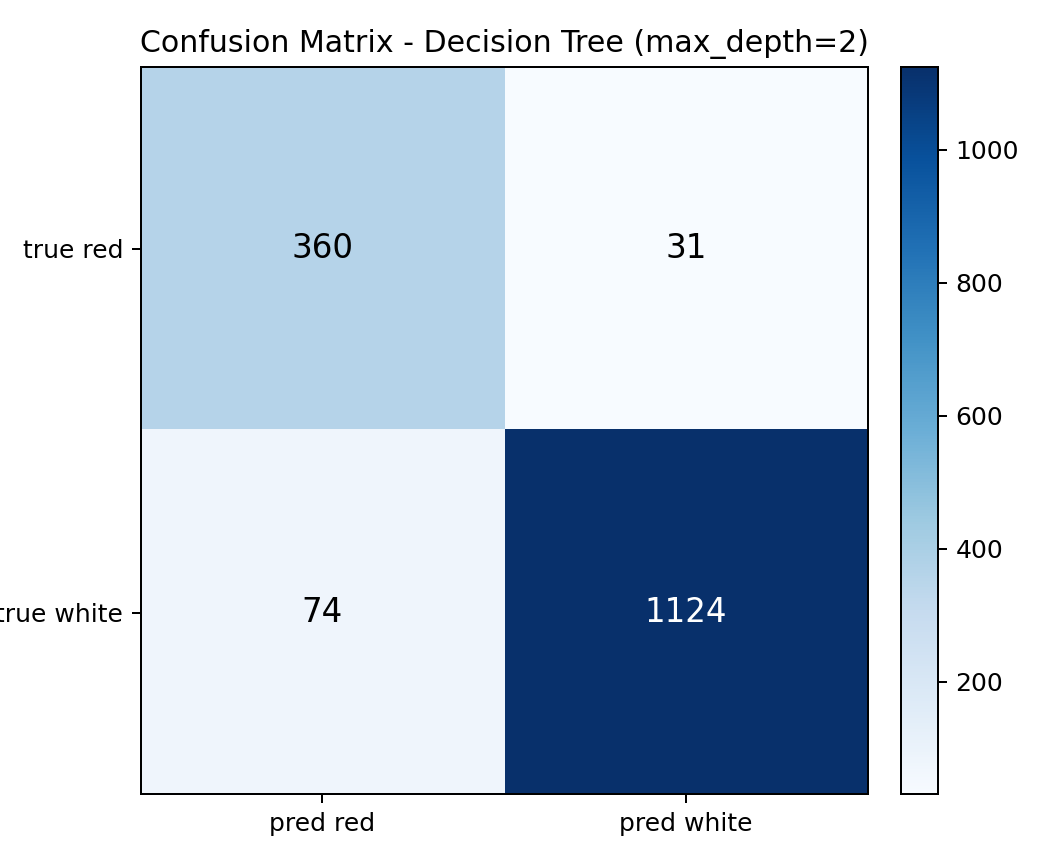
\includegraphics[width=0.62\textwidth]{q1_confusion_matrix.png}
\caption{Confusion matrix του δέντρου ταξινόμησης.}
\end{figure}

\begin{figure}[H]
\centering
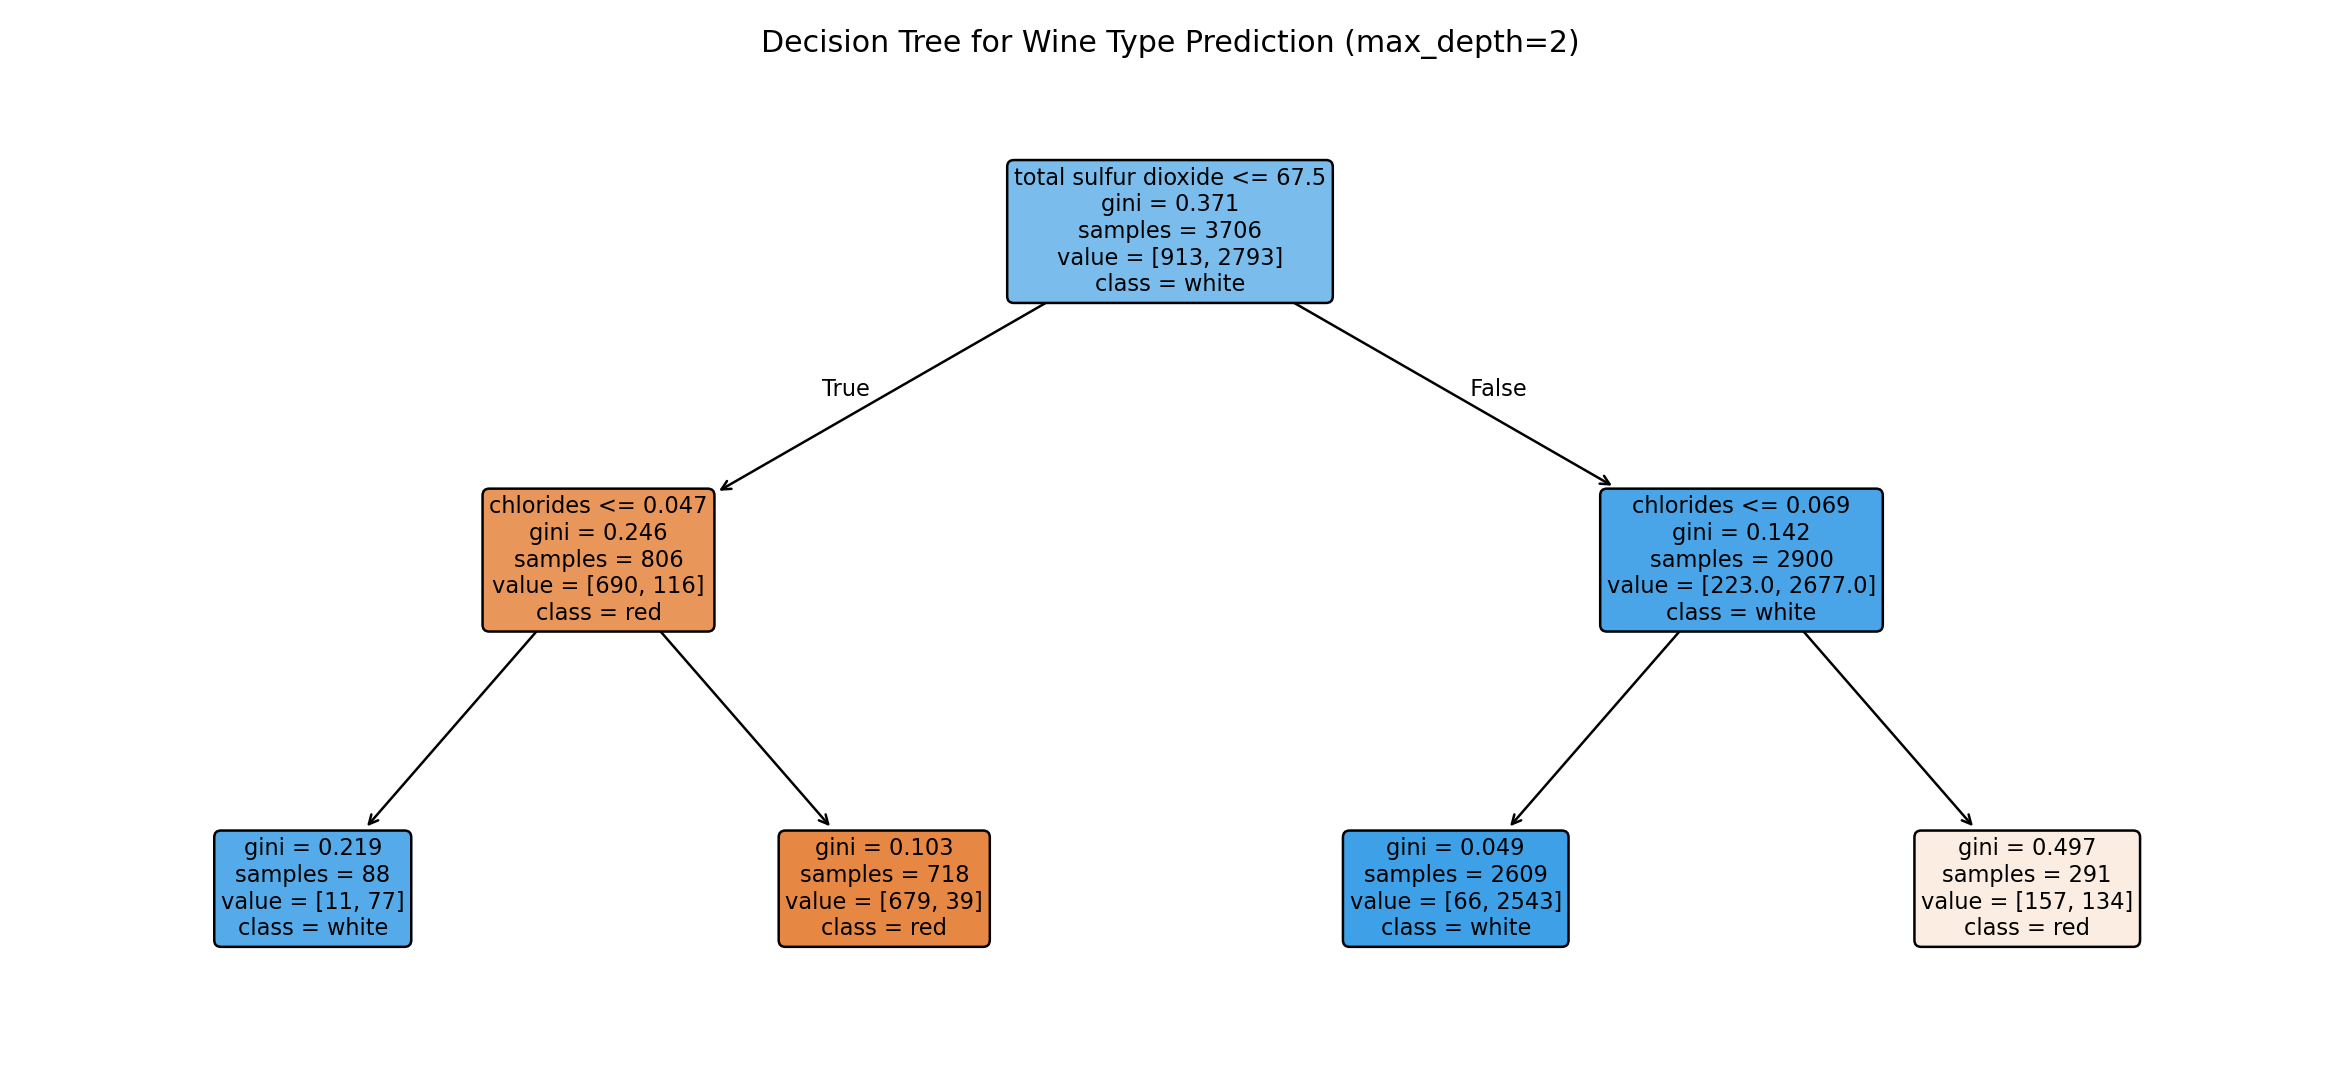
\includegraphics[width=\textwidth]{q1_decision_tree_plot.png}
\caption{Το δέντρο ταξινόμησης με μέγιστο βάθος 2.}
\end{figure}

\subsection{Ερμηνεία}

Το δέντρο βασίστηκε κυρίως στις μεταβλητές \code{total sulfur dioxide} και
\code{chlorides}. Οι κανόνες του ήταν:

\begin{verbatim}
total sulfur dioxide <= 67.50
|-- chlorides <= 0.05  -> white
|-- chlorides >  0.05  -> red

total sulfur dioxide > 67.50
|-- chlorides <= 0.07  -> white
|-- chlorides >  0.07  -> red
\end{verbatim}

Οι τιμές που εμφανίζονται στους κανόνες δεν επιλέχθηκαν από εμάς αυθαίρετα.
Τις επέλεξε ο αλγόριθμος κατά την εκπαίδευση του δέντρου. Πιο συγκεκριμένα,
τα πραγματικά thresholds ήταν 67.50 για τη \code{total sulfur dioxide},
0.0475 για τη \code{chlorides} στον αριστερό κόμβο και 0.0695 για τη
\code{chlorides} στον δεξιό κόμβο. Στο κείμενο των κανόνων οι δύο τελευταίες
τιμές εμφανίζονται στρογγυλοποιημένες ως 0.05 και 0.07.

Το \code{DecisionTreeClassifier} δοκιμάζει πιθανούς διαχωρισμούς των
μεταβλητών και επιλέγει εκείνους που κάνουν τις ομάδες όσο γίνεται πιο
«καθαρές» ως προς την κλάση \code{red}/\code{white}. Με την προεπιλεγμένη
ρύθμιση του scikit-learn, αυτό γίνεται με βάση το κριτήριο
\textenglish{Gini impurity}.

Επειδή έχουμε κωδικοποιήσει \code{red=0} και \code{white=1}, όταν στους κανόνες
εμφανίζεται \code{class: 0} σημαίνει πρόβλεψη κόκκινου κρασιού, ενώ
\code{class: 1} σημαίνει πρόβλεψη λευκού κρασιού.

Το μοντέλο πέτυχε accuracy 0.9339, δηλαδή ταξινόμησε σωστά περίπου το 93.39\%
των test παρατηρήσεων. Αυτό είναι αρκετά καλό αποτέλεσμα, ειδικά επειδή το
δέντρο είναι πολύ απλό.

%=============================================================================
\section{Ερώτημα 2: Bagging με 200 εκτιμητές}
%=============================================================================

\subsection{Τι ζητάει το ερώτημα}

Το δεύτερο ερώτημα είναι:

\begin{quote}
\textbf{«Να γίνει πρόβλεψη/εκτίμηση του τύπου κρασιού με τη μέθοδο Bagging,
χρησιμοποιώντας 200 εκτιμητές.»}
\end{quote}

Εδώ δεν χρησιμοποιούμε ένα μόνο δέντρο. Χρησιμοποιούμε 200 δέντρα και
συνδυάζουμε τις προβλέψεις τους. Αυτό είναι το βασικό σημείο του ερωτήματος:
αντί να εμπιστευτούμε μία μόνο απόφαση, φτιάχνουμε πολλές διαφορετικές
εκδοχές δέντρων και αφήνουμε την πλειοψηφία να αποφασίσει.

Πρακτικά, το ερώτημα μάς ζητά να απαντήσουμε στο εξής:

\begin{quote}
Αν το απλό δέντρο του Ερωτήματος 1 είχε κάποια λάθη, μπορούμε να βελτιώσουμε
την πρόβλεψη χρησιμοποιώντας πολλά δέντρα αντί για ένα;
\end{quote}

\subsection{Η πιο απλή ιδέα του Bagging}

Ας το πούμε όσο πιο απλά γίνεται.

Στο Ερώτημα 1 είχαμε \textbf{ένα} δέντρο. Δηλαδή ήταν σαν να ρωτάμε έναν μόνο
«κριτή»:

\begin{quote}
Αυτό το κρασί είναι κόκκινο ή λευκό;
\end{quote}

Ο ένας κριτής μπορεί να κάνει λάθος. Για παράδειγμα, μπορεί να μπερδευτεί σε
κάποια κρασιά που μοιάζουν χημικά μεταξύ τους.

Στο Bagging δεν ρωτάμε έναν μόνο κριτή. Ρωτάμε \textbf{200 δέντρα}. Κάθε
δέντρο δίνει τη δική του απάντηση και στο τέλος κρατάμε την απάντηση που
ψήφισαν τα περισσότερα δέντρα.

Άρα, για ένα κρασί, μπορεί να γίνει κάτι τέτοιο:

\begin{center}
\begin{tabular}{lr}
\toprule
\textbf{Τι ψήφισαν τα δέντρα} & \textbf{Πλήθος ψήφων} \\
\midrule
\code{white} & 160 \\
\code{red} & 40 \\
\bottomrule
\end{tabular}
\end{center}

Επειδή τα περισσότερα δέντρα ψήφισαν \code{white}, το Bagging θα προβλέψει
\code{white}.

Αυτή είναι η κεντρική ιδέα:

\begin{quote}
\textbf{Το Bagging είναι σαν να βάζουμε πολλά δέντρα να ψηφίσουν, αντί να
αποφασίζει μόνο ένα δέντρο.}
\end{quote}

\subsection{Από πού βγαίνουν τα 200 διαφορετικά δέντρα}

Ίσως το πιο μπερδεμένο σημείο είναι αυτό: αφού έχουμε ένα training set, πώς
φτιάχνουμε 200 διαφορετικά δέντρα;

Δεν χωρίζουμε τα δεδομένα 200 φορές σε training και test. Αυτό θα ήταν άλλο
πράγμα. Το test set παραμένει το ίδιο και το χρησιμοποιούμε μόνο στο τέλος.

Αυτό που κάνει το Bagging είναι το εξής:

\begin{enumerate}
    \item Παίρνει το training set.
    \item Φτιάχνει από αυτό ένα «τυχαίο αντίγραφο» με δειγματοληψία με
    επανάθεση.
    \item Εκπαιδεύει ένα δέντρο σε αυτό το τυχαίο αντίγραφο.
    \item Ξανακάνει την ίδια διαδικασία 200 φορές.
\end{enumerate}

Το «με επανάθεση» σημαίνει ότι όταν διαλέγουμε μία γραμμή από το training set,
μπορούμε να τη διαλέξουμε ξανά. Έτσι κάθε τυχαίο αντίγραφο είναι λίγο
διαφορετικό από τα υπόλοιπα.

Ένα μικρό παράδειγμα:

\begin{center}
Αρχικό training set: A, B, C, D, E
\end{center}

Ένα bootstrap δείγμα μπορεί να είναι:

\begin{center}
A, C, C, E, B
\end{center}

Ένα άλλο bootstrap δείγμα μπορεί να είναι:

\begin{center}
B, B, D, E, A
\end{center}

Βλέπουμε ότι τα δείγματα μοιάζουν, αλλά δεν είναι ακριβώς ίδια. Έτσι και τα
δέντρα που εκπαιδεύονται πάνω τους δεν είναι ακριβώς ίδια.

\subsection{Άρα τι έκανε το Bagging στη δική μας εργασία}

Στη δική μας εργασία έγινε αυτό:

\begin{enumerate}
    \item Χωρίσαμε τα δεδομένα μία φορά σε training και test.
    \item Το training set είχε 3706 κρασιά.
    \item Το Bagging έφτιαξε 200 τυχαία bootstrap δείγματα από αυτά τα 3706
    training κρασιά.
    \item Εκπαίδευσε 200 δέντρα, ένα για κάθε bootstrap δείγμα.
    \item Μετά πήρε τα 1589 test κρασιά.
    \item Για κάθε test κρασί, τα 200 δέντρα ψήφισαν \code{red} ή \code{white}.
    \item Η τελική πρόβλεψη ήταν η πλειοψηφία των ψήφων.
\end{enumerate}

Αν το πούμε σε μία πρόταση:

\begin{quote}
Το Bagging φτιάχνει πολλά λίγο διαφορετικά δέντρα και τα βάζει να ψηφίσουν.
\end{quote}

\subsection{Θεωρητικό υπόβαθρο}

Το Bagging προέρχεται από τη φράση \textenglish{Bootstrap Aggregating}. Η
βασική ιδέα είναι:

\begin{enumerate}
    \item Δημιουργούμε πολλά bootstrap δείγματα από το training set.
    \item Εκπαιδεύουμε ένα δέντρο σε κάθε bootstrap δείγμα.
    \item Κάθε δέντρο κάνει τη δική του πρόβλεψη.
    \item Η τελική πρόβλεψη προκύπτει με πλειοψηφική ψηφοφορία.
\end{enumerate}

Ένα bootstrap δείγμα δημιουργείται με δειγματοληψία \textbf{με επανάθεση}.
Αυτό σημαίνει ότι μία παρατήρηση μπορεί να εμφανιστεί περισσότερες από μία
φορές στο ίδιο bootstrap δείγμα, ενώ κάποια άλλη παρατήρηση μπορεί να μην
εμφανιστεί καθόλου.

Για να γίνει πιο κατανοητό, ας φανταστούμε ένα μικρό training set με πέντε
παρατηρήσεις:

\begin{center}
A, B, C, D, E.
\end{center}

Ένα bootstrap δείγμα ίδιου μεγέθους θα μπορούσε να είναι:

\begin{center}
A, C, C, E, B.
\end{center}

Εδώ η παρατήρηση C εμφανίστηκε δύο φορές, ενώ η D δεν εμφανίστηκε καθόλου.
Αυτό δεν είναι λάθος. Είναι ακριβώς η ιδέα της δειγματοληψίας με επανάθεση.

\subsection{Τι ακριβώς κάνει το Bagging στα δικά μας δεδομένα}

Στα δικά μας δεδομένα, το training set έχει 3706 παρατηρήσεις. Όταν
χρησιμοποιούμε Bagging με \code{n\_estimators=200}, η διαδικασία είναι:

\begin{enumerate}
    \item Δημιουργείται ένα bootstrap δείγμα από το training set.
    \item Εκπαιδεύεται ένα δέντρο ταξινόμησης σε αυτό το δείγμα.
    \item Η διαδικασία επαναλαμβάνεται 200 φορές.
    \item Έτσι προκύπτουν 200 διαφορετικά δέντρα.
    \item Για κάθε παρατήρηση του test set, τα 200 δέντρα ψηφίζουν αν είναι
    \code{red} ή \code{white}.
    \item Η τελική πρόβλεψη είναι η κλάση με τις περισσότερες ψήφους.
\end{enumerate}

Ένα σημαντικό σημείο είναι ότι \textbf{δεν κάνουμε 200 διαφορετικούς
διαχωρισμούς σε training και test set}. Το training/test split γίνεται μία
φορά, όπως και στα υπόλοιπα ερωτήματα. Τα 200 δείγματα δημιουργούνται μόνο
μέσα από το training set.

\subsection{Πώς γίνεται η τελική ψηφοφορία}

Επειδή έχουμε πρόβλημα ταξινόμησης, το Bagging χρησιμοποιεί πλειοψηφική
ψηφοφορία. Για κάθε κρασί του test set, κάθε ένα από τα 200 δέντρα δίνει μία
πρόβλεψη.

Για παράδειγμα, για ένα συγκεκριμένο κρασί μπορεί να έχουμε:

\begin{center}
\begin{tabular}{lr}
\toprule
\textbf{Πρόβλεψη} & \textbf{Πλήθος δέντρων} \\
\midrule
\code{white} & 173 \\
\code{red} & 27 \\
\bottomrule
\end{tabular}
\end{center}

Σε αυτή την περίπτωση, η τελική πρόβλεψη του Bagging είναι \code{white}, επειδή
τα περισσότερα δέντρα ψήφισαν \code{white}.

Αντίστοιχα, αν τα περισσότερα δέντρα ψήφιζαν \code{red}, η τελική πρόβλεψη θα
ήταν \code{red}.

\subsection{Γιατί το Bagging βοηθά τα δέντρα}

Τα δέντρα ταξινόμησης είναι εύχρηστα και ερμηνεύσιμα, αλλά έχουν ένα γνωστό
μειονέκτημα: μπορούν να είναι ασταθή. Μικρές αλλαγές στα training δεδομένα
μπορεί να οδηγήσουν σε διαφορετικό δέντρο.

Το Bagging μειώνει αυτό το πρόβλημα επειδή δεν βασίζεται σε ένα μόνο δέντρο.
Αντίθετα, δημιουργεί πολλά δέντρα σε διαφορετικά bootstrap δείγματα. Κάθε
δέντρο μπορεί να έχει τα δικά του λάθη, αλλά όταν συνδυάζουμε 200 δέντρα, τα
τυχαία λάθη τείνουν να εξομαλύνονται.

Με απλά λόγια:

\begin{quote}
Το Bagging δεν κάνει απαραίτητα κάθε δέντρο καλύτερο. Κάνει όμως την τελική
απόφαση πιο σταθερή, επειδή βασίζεται στη συλλογική απόφαση πολλών δέντρων.
\end{quote}

\begin{figure}[H]
\centering
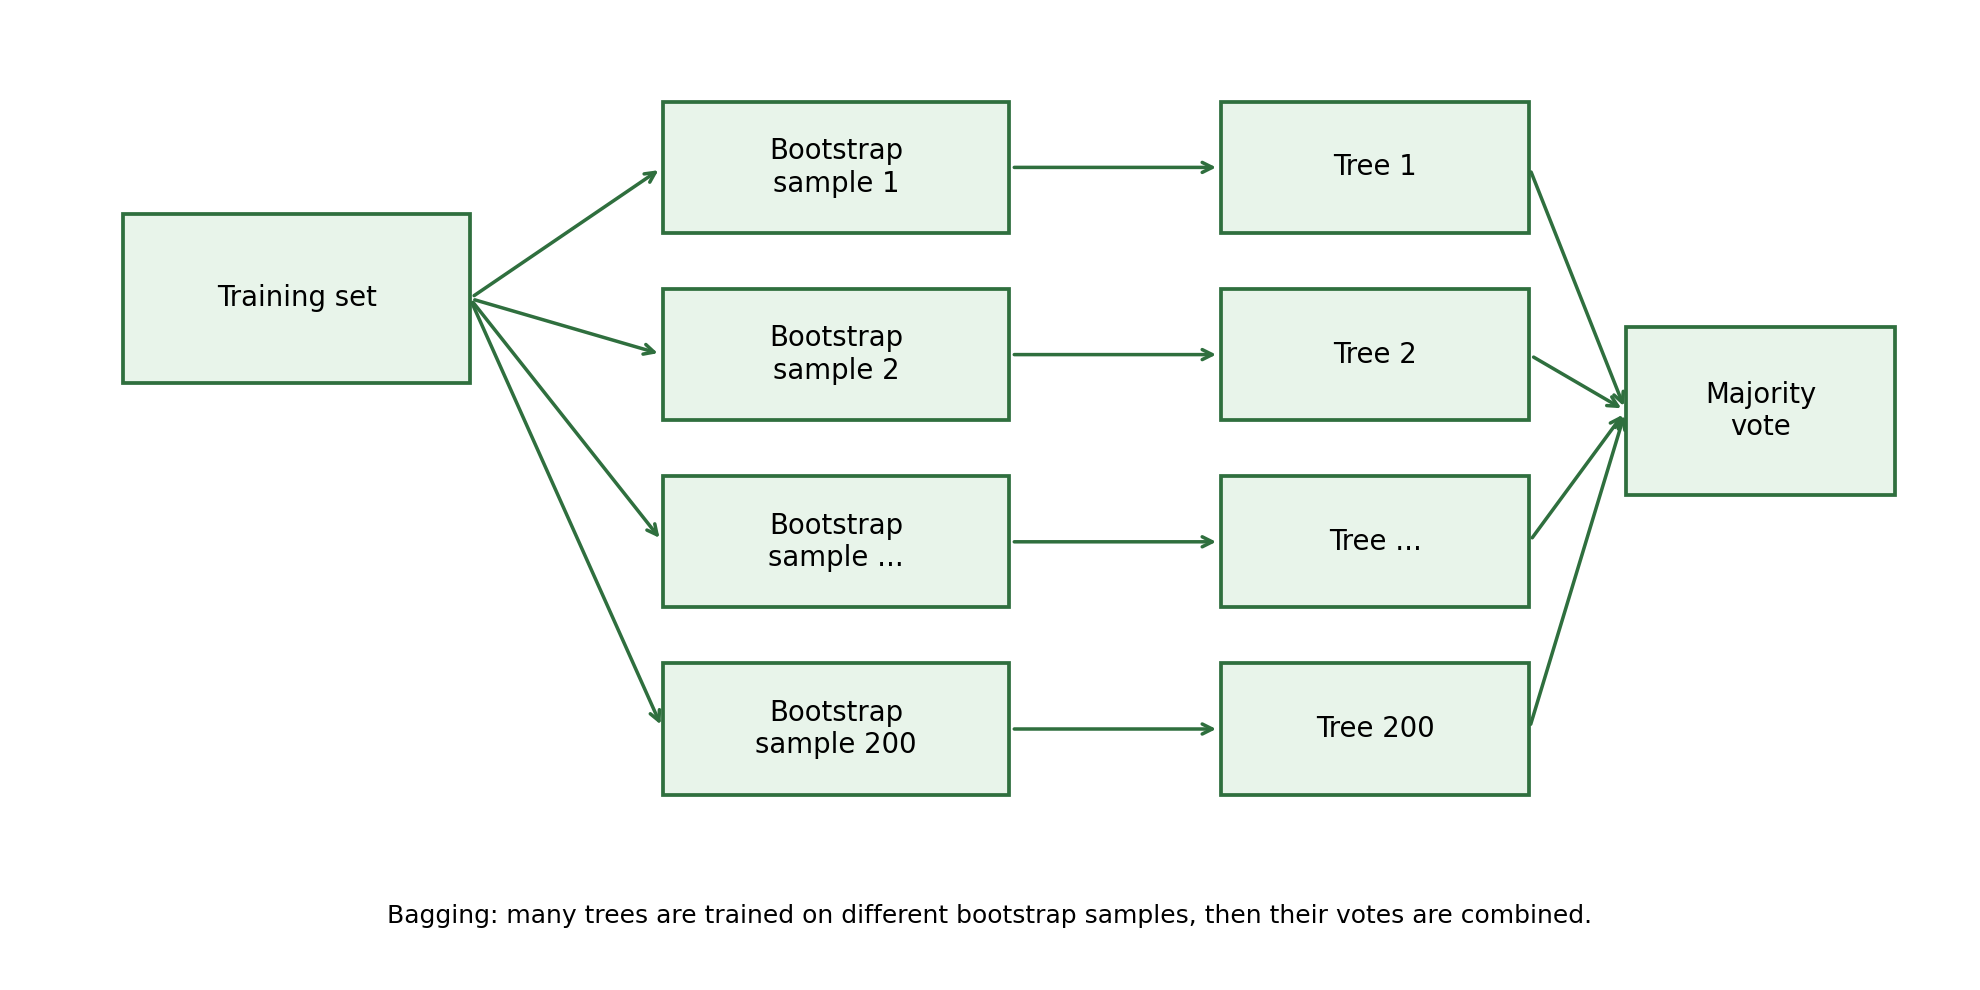
\includegraphics[width=0.92\textwidth]{q2_bagging_concept.png}
\caption{Η βασική ιδέα του Bagging.}
\end{figure}

\subsection{Πώς το λύσαμε}

Χρησιμοποιήσαμε τον ίδιο διαχωρισμό training/test με το Ερώτημα 1, ώστε η
σύγκριση να είναι δίκαιη. Αν αλλάζαμε το test set, δεν θα ξέραμε αν η διαφορά
στην απόδοση οφείλεται στο μοντέλο ή απλώς σε διαφορετικά test δεδομένα.

Οι predictors και η μεταβλητή στόχος ορίστηκαν όπως πριν:

\begin{lstlisting}[language=Python]
features = [col for col in df.columns if col not in ("quality", "wine_type")]
X = df[features]
y = (df["wine_type"] == "white").astype(int)
\end{lstlisting}

Στη συνέχεια έγινε το ίδιο train/test split:

\begin{lstlisting}[language=Python]
X_train, X_test, y_train, y_test = train_test_split(
    X,
    y,
    test_size=0.30,
    random_state=6931,
    stratify=y,
)
\end{lstlisting}

Το Bagging μοντέλο ορίστηκε ως:

\begin{lstlisting}[language=Python]
model = BaggingClassifier(
    estimator=DecisionTreeClassifier(random_state=6931),
    n_estimators=200,
    random_state=6931,
    n_jobs=-1,
)
\end{lstlisting}

Ας εξηγήσουμε αναλυτικά τις παραμέτρους:

\begin{itemize}
    \item \code{BaggingClassifier}: δηλώνει ότι χρησιμοποιούμε Bagging για
    ταξινόμηση.
    \item \code{estimator=DecisionTreeClassifier(...)}: δηλώνει ότι το κάθε
    επιμέρους μοντέλο είναι δέντρο ταξινόμησης.
    \item \code{n\_estimators=200}: δηλώνει ότι θα δημιουργηθούν και θα
    εκπαιδευτούν 200 δέντρα.
    \item \code{random\_state=6931}: κάνει τη διαδικασία αναπαραγώγιμη.
    \item \code{n\_jobs=-1}: επιτρέπει τη χρήση όλων των διαθέσιμων πυρήνων
    του υπολογιστή για ταχύτερη εκτέλεση.
\end{itemize}

Έπειτα εκπαιδεύσαμε το μοντέλο:

\begin{lstlisting}[language=Python]
model.fit(X_train, y_train)
\end{lstlisting}

Με αυτή την εντολή, το Bagging δημιούργησε τα 200 bootstrap δείγματα και
εκπαίδευσε τα 200 δέντρα.

Τέλος, κάναμε προβλέψεις στο test set:

\begin{lstlisting}[language=Python]
y_pred = model.predict(X_test)
accuracy = accuracy_score(y_test, y_pred)
test_error = 1 - accuracy
\end{lstlisting}

Η μεταβλητή \code{y\_pred} περιέχει την τελική πρόβλεψη του Bagging για κάθε
test παρατήρηση, δηλαδή το αποτέλεσμα της πλειοψηφικής ψηφοφορίας των 200
δέντρων.

\subsection{Αποτελέσματα}

\begin{table}[H]
\centering
\caption{Αποτελέσματα Bagging με 200 εκτιμητές.}
\begin{tabular}{lr}
\toprule
\textbf{Μέτρο} & \textbf{Τιμή} \\
\midrule
Test accuracy & 0.9660 \\
Test error & 0.0340 \\
Σωστές προβλέψεις & 1535 \\
Λανθασμένες προβλέψεις & 54 \\
\bottomrule
\end{tabular}
\end{table}

Ο confusion matrix ήταν:

\begin{table}[H]
\centering
\caption{Confusion matrix για το Bagging.}
\begin{tabular}{lcc}
\toprule
& \textbf{Πρόβλεψη red} & \textbf{Πρόβλεψη white} \\
\midrule
\textbf{Πραγματικό red} & 365 & 26 \\
\textbf{Πραγματικό white} & 28 & 1170 \\
\bottomrule
\end{tabular}
\end{table}

\subsection{Πώς προκύπτουν οι αριθμοί του Bagging}

Ο confusion matrix συγκρίνει την πραγματική κλάση κάθε test παρατήρησης με την
πρόβλεψη του Bagging. Τα τέσσερα κελιά του πίνακα σημαίνουν:

\begin{itemize}
    \item \textbf{365}: κόκκινα κρασιά που προβλέφθηκαν σωστά ως κόκκινα.
    \item \textbf{26}: κόκκινα κρασιά που προβλέφθηκαν λάθος ως λευκά.
    \item \textbf{28}: λευκά κρασιά που προβλέφθηκαν λάθος ως κόκκινα.
    \item \textbf{1170}: λευκά κρασιά που προβλέφθηκαν σωστά ως λευκά.
\end{itemize}

Άρα στο test set είχαμε:

\[
    365 + 26 = 391
\]

κόκκινα κρασιά και:

\[
    28 + 1170 = 1198
\]

λευκά κρασιά. Συνολικά:

\[
    391 + 1198 = 1589
\]

test παρατηρήσεις.

Οι σωστές προβλέψεις είναι τα κελιά της κύριας διαγωνίου:

\[
    365 + 1170 = 1535.
\]

Τα λάθη είναι τα δύο εκτός διαγωνίου κελιά:

\[
    26 + 28 = 54.
\]

Άρα η test accuracy είναι:

\[
    \text{Test Accuracy}
    =
    \frac{1535}{1589}
    =
    0.9660.
\]

Και το test error είναι:

\[
    \text{Test Error}
    =
    \frac{54}{1589}
    =
    0.0340.
\]

Επομένως, το Bagging έκανε σωστή πρόβλεψη για 1535 από τα 1589 κρασιά του test
set και λάθος πρόβλεψη για 54 κρασιά.

\begin{figure}[H]
\centering
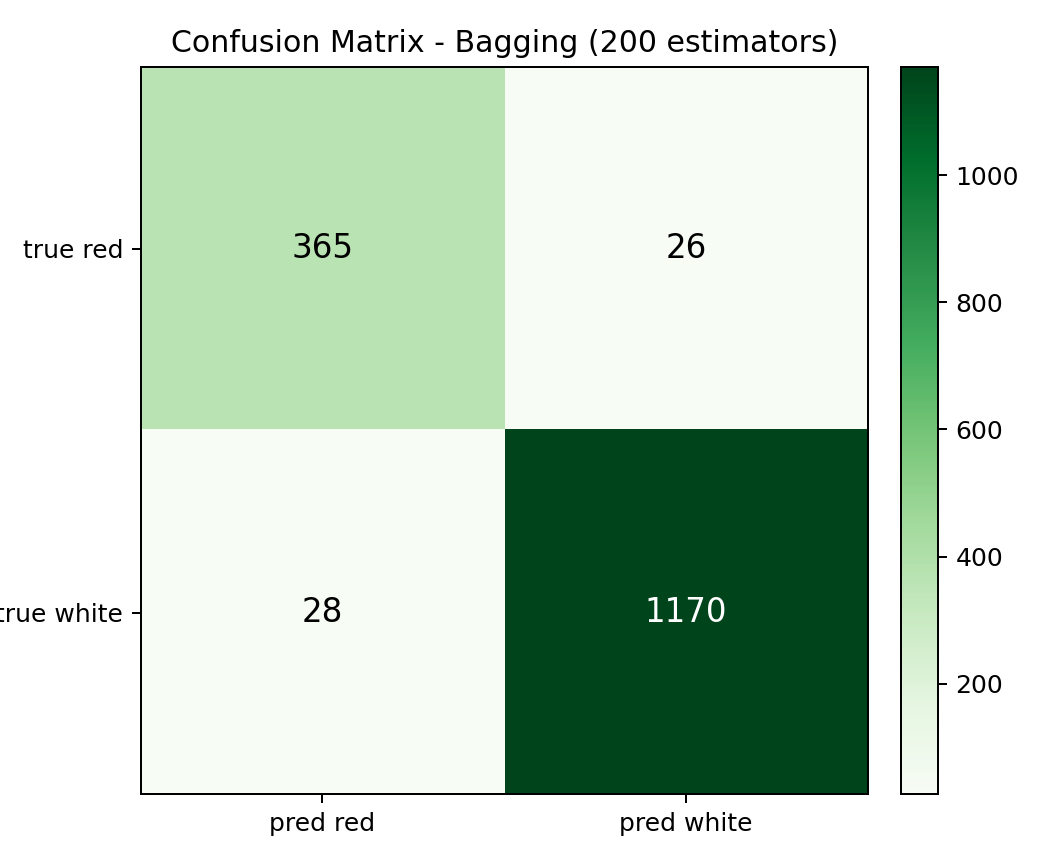
\includegraphics[width=0.62\textwidth]{q2_confusion_matrix.png}
\caption{Confusion matrix του Bagging.}
\end{figure}

\subsection{Σύγκριση με το Ερώτημα 1}

\begin{table}[H]
\centering
\caption{Σύγκριση απλού δέντρου και Bagging.}
\begin{tabular}{lrr}
\toprule
\textbf{Μοντέλο} & \textbf{Test Accuracy} & \textbf{Test Error} \\
\midrule
Decision Tree (\code{max\_depth=2}) & 0.9339 & 0.0661 \\
Bagging (200 estimators) & 0.9660 & 0.0340 \\
\bottomrule
\end{tabular}
\end{table}

Το Bagging έκανε 54 λάθη, ενώ το απλό δέντρο έκανε 105 λάθη. Άρα το Bagging
έκανε:

\[
    105 - 54 = 51
\]

λιγότερα λάθη.

Μπορούμε να δούμε τη βελτίωση και ως διαφορά στην accuracy:

\[
    0.9660 - 0.9339 = 0.0321.
\]

Δηλαδή το Bagging αύξησε την ακρίβεια κατά περίπου 3.21 ποσοστιαίες μονάδες.
Σε επίπεδο test error, η μείωση είναι:

\[
    0.0661 - 0.0340 = 0.0321.
\]

Άρα το σφάλμα σχεδόν υποδιπλασιάστηκε. Το απλό δέντρο έκανε λάθος περίπου στο
6.61\% των test παρατηρήσεων, ενώ το Bagging έκανε λάθος περίπου στο 3.40\%.

\subsection{Γιατί το Bagging βελτιώθηκε τόσο σε σχέση με το απλό δέντρο}

Το απλό δέντρο του Ερωτήματος 1 είχε \code{max\_depth=2}, άρα ήταν πολύ
περιορισμένο. Μπορούσε να χρησιμοποιήσει λίγους μόνο κανόνες. Αυτό το έκανε
εύκολα ερμηνεύσιμο, αλλά ταυτόχρονα περιόριζε την προβλεπτική του δύναμη.

Το Bagging, αντίθετα, χρησιμοποίησε πολλά δέντρα. Κάθε δέντρο εκπαιδεύτηκε σε
διαφορετικό bootstrap δείγμα και μπορούσε να αποτυπώσει διαφορετικές πλευρές
των δεδομένων. Η τελική ψηφοφορία των 200 δέντρων ήταν πιο αξιόπιστη από την
απόφαση ενός μόνο δέντρου.

Αυτό εξηγεί γιατί τα λάθη μειώθηκαν από 105 σε 54. Δεν σημαίνει ότι κάθε ένα
από τα 200 δέντρα ήταν τέλειο. Σημαίνει ότι ο συνδυασμός τους έδωσε πιο
σταθερό και ακριβές αποτέλεσμα.

\subsection{Σημαντικότητα χαρακτηριστικών}

\begin{figure}[H]
\centering
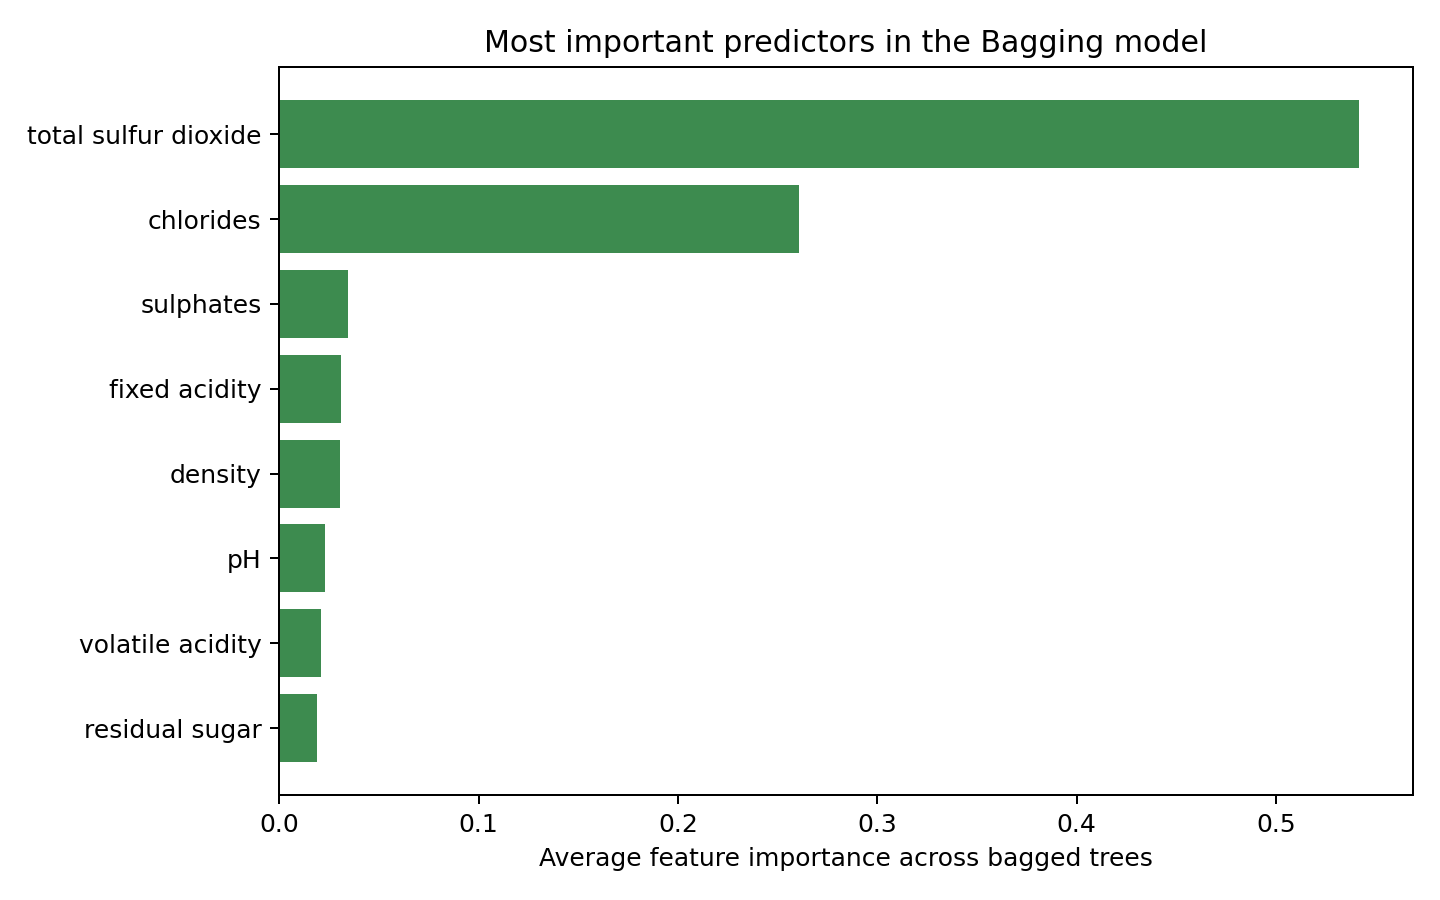
\includegraphics[width=0.82\textwidth]{q2_bagging_feature_importance.png}
\caption{Οι σημαντικότερες μεταβλητές στο Bagging.}
\end{figure}

Οι σημαντικότερες μεταβλητές στο Bagging ήταν κυρίως οι
\code{total sulfur dioxide} και \code{chlorides}. Αυτό συμφωνεί με το απλό
δέντρο του Ερωτήματος 1.

\begin{table}[H]
\centering
\caption{Μέση σημαντικότητα χαρακτηριστικών στο Bagging.}
\small
\begin{tabular}{lr}
\toprule
\textbf{Μεταβλητή} & \textbf{Σημαντικότητα} \\
\midrule
\code{total sulfur dioxide} & 0.5416 \\
\code{chlorides} & 0.2609 \\
\code{sulphates} & 0.0347 \\
\code{fixed acidity} & 0.0312 \\
\code{density} & 0.0303 \\
\code{pH} & 0.0228 \\
\code{volatile acidity} & 0.0211 \\
\code{residual sugar} & 0.0187 \\
\code{citric acid} & 0.0139 \\
\code{alcohol} & 0.0135 \\
\code{free sulfur dioxide} & 0.0112 \\
\bottomrule
\end{tabular}
\end{table}

Η σημαντικότητα χαρακτηριστικών δεν σημαίνει ότι οι υπόλοιπες μεταβλητές δεν
χρησιμοποιήθηκαν ποτέ. Σημαίνει ότι, κατά μέσο όρο στα 200 δέντρα, οι
μεταβλητές \code{total sulfur dioxide} και \code{chlorides} συνέβαλαν
περισσότερο στους διαχωρισμούς που μείωναν την ακαθαρσία των κόμβων.

\subsection{Συμπέρασμα Ερωτήματος 2}

Το Bagging με 200 εκτιμητές πέτυχε test accuracy 0.9660. Η απόδοση είναι
σημαντικά καλύτερη από το απλό δέντρο, επειδή το Bagging δεν βασίζεται σε ένα
μόνο δέντρο αλλά σε ψηφοφορία πολλών δέντρων.

Το βασικό συμπέρασμα είναι ότι η χρήση πολλών bootstrap δειγμάτων και πολλών
δέντρων μειώνει την αστάθεια ενός μεμονωμένου δέντρου. Έτσι, το μοντέλο κάνει
λιγότερα λάθη στο test set και γενικεύει καλύτερα. Για αυτό το Bagging είναι
μία από τις πιο κλασικές τεχνικές βελτίωσης των δέντρων απόφασης.

%=============================================================================
\section{Ερώτημα 3: Random Forest με 200 εκτιμητές και \texorpdfstring{$m=p/2$}{m=p/2}}
%=============================================================================

\subsection{Τι ζητάει το ερώτημα}

Το τρίτο ερώτημα είναι:

\begin{quote}
\textbf{«Να γίνει πρόβλεψη/εκτίμηση του τύπου κρασιού με Random Forest,
χρησιμοποιώντας 200 εκτιμητές και τυχαίο πλήθος υποψήφιων χαρακτηριστικών
$m=p/2$.»}
\end{quote}

Εδώ χρησιμοποιούμε ξανά πολλά δέντρα, όπως στο Bagging. Η διαφορά είναι ότι
στο Random Forest κάθε split κάθε δέντρου δεν εξετάζει όλες τις μεταβλητές,
αλλά μόνο ένα τυχαίο υποσύνολο.

Με πολύ απλά λόγια, το ερώτημα δεν ζητά να φτιάξουμε ένα μόνο δέντρο.
Ζητά να φτιάξουμε ένα \textbf{δάσος} από 200 δέντρα αποφάσεων. Κάθε δέντρο
δίνει τη δική του πρόβλεψη για το αν ένα κρασί είναι κόκκινο ή λευκό, και στο
τέλος κρατάμε την απάντηση που ψήφισαν τα περισσότερα δέντρα.

Το επιπλέον σημείο που πρέπει να προσέξουμε είναι το $m=p/2$. Αυτό σημαίνει
ότι, όταν ένα δέντρο προσπαθεί να αποφασίσει σε ποια μεταβλητή θα κάνει split,
δεν κοιτάζει όλες τις διαθέσιμες μεταβλητές. Κοιτάζει μόνο ένα τυχαίο
υποσύνολο μεταβλητών. Έτσι τα δέντρα δεν γίνονται όλα ίδια μεταξύ τους.

\subsection{Θεωρητικό υπόβαθρο}

Το Random Forest είναι σαν Bagging, αλλά με επιπλέον τυχαιότητα. Για να το
καταλάβουμε σωστά, ας το δούμε σε σχέση με αυτά που κάναμε στο προηγούμενο
ερώτημα.

Στο Bagging:

\begin{itemize}
    \item παίρναμε πολλά bootstrap δείγματα από το training set,
    \item εκπαιδεύαμε ένα δέντρο σε κάθε bootstrap δείγμα,
    \item συνδυάζαμε τις προβλέψεις των δέντρων με ψηφοφορία.
\end{itemize}

Στο Random Forest κάνουμε τα ίδια, αλλά προσθέτουμε μία ακόμα ιδέα:

\begin{itemize}
    \item κάθε δέντρο εξακολουθεί να εκπαιδεύεται σε bootstrap δείγμα,
    \item όμως σε κάθε split εξετάζεται μόνο τυχαίο υποσύνολο χαρακτηριστικών,
    \item από αυτό το μικρότερο υποσύνολο επιλέγεται το καλύτερο split,
    \item στο τέλος όλα τα δέντρα ψηφίζουν για την τελική κλάση.
\end{itemize}

Αυτό βοηθά γιατί κάνει τα δέντρα πιο διαφορετικά μεταξύ τους. Αν όλα τα δέντρα
μοιάζουν πολύ, τότε μπορεί να κάνουν παρόμοια λάθη. Αν όμως είναι πιο
διαφορετικά, η πλειοψηφική ψηφοφορία γίνεται πιο χρήσιμη.

\subsection{Γιατί δεν αρκεί πάντα το Bagging}

Στο Bagging, κάθε δέντρο μπορεί να εξετάσει όλες τις μεταβλητές σε κάθε split.
Αν υπάρχει μία πολύ δυνατή μεταβλητή, όπως για παράδειγμα η
\code{total sulfur dioxide}, πολλά δέντρα είναι πιθανό να τη χρησιμοποιήσουν
πολύ νωρίς. Αυτό κάνει τα δέντρα καλύτερα μεμονωμένα, αλλά μπορεί να τα κάνει
και αρκετά παρόμοια μεταξύ τους.

Το πρόβλημα είναι το εξής: αν τα 200 δέντρα μοιάζουν πολύ μεταξύ τους, τότε τα
200 δέντρα δεν μας δίνουν 200 πραγματικά διαφορετικές απόψεις. Είναι σαν να
ρωτάμε πολλούς ανθρώπους που σκέφτονται σχεδόν με τον ίδιο τρόπο.

Το Random Forest προσπαθεί να μειώσει αυτό το πρόβλημα. Σε κάθε split λέει στο
δέντρο:

\begin{quote}
«Μην κοιτάξεις όλες τις μεταβλητές. Θα σου δώσω τυχαία μόνο μερικές από αυτές.
Διάλεξε το καλύτερο split μόνο ανάμεσα σε αυτές.»
\end{quote}

Έτσι, αν σε κάποιο split δεν τύχει να είναι διαθέσιμη η πιο δυνατή μεταβλητή,
το δέντρο αναγκάζεται να βρει καλή πληροφορία από κάποια άλλη μεταβλητή. Αυτό
δημιουργεί πιο διαφορετικά δέντρα. Και όταν τα δέντρα είναι πιο διαφορετικά, η
ψηφοφορία τους μπορεί να γενικεύει καλύτερα σε άγνωστα δεδομένα.

\begin{figure}[H]
\centering
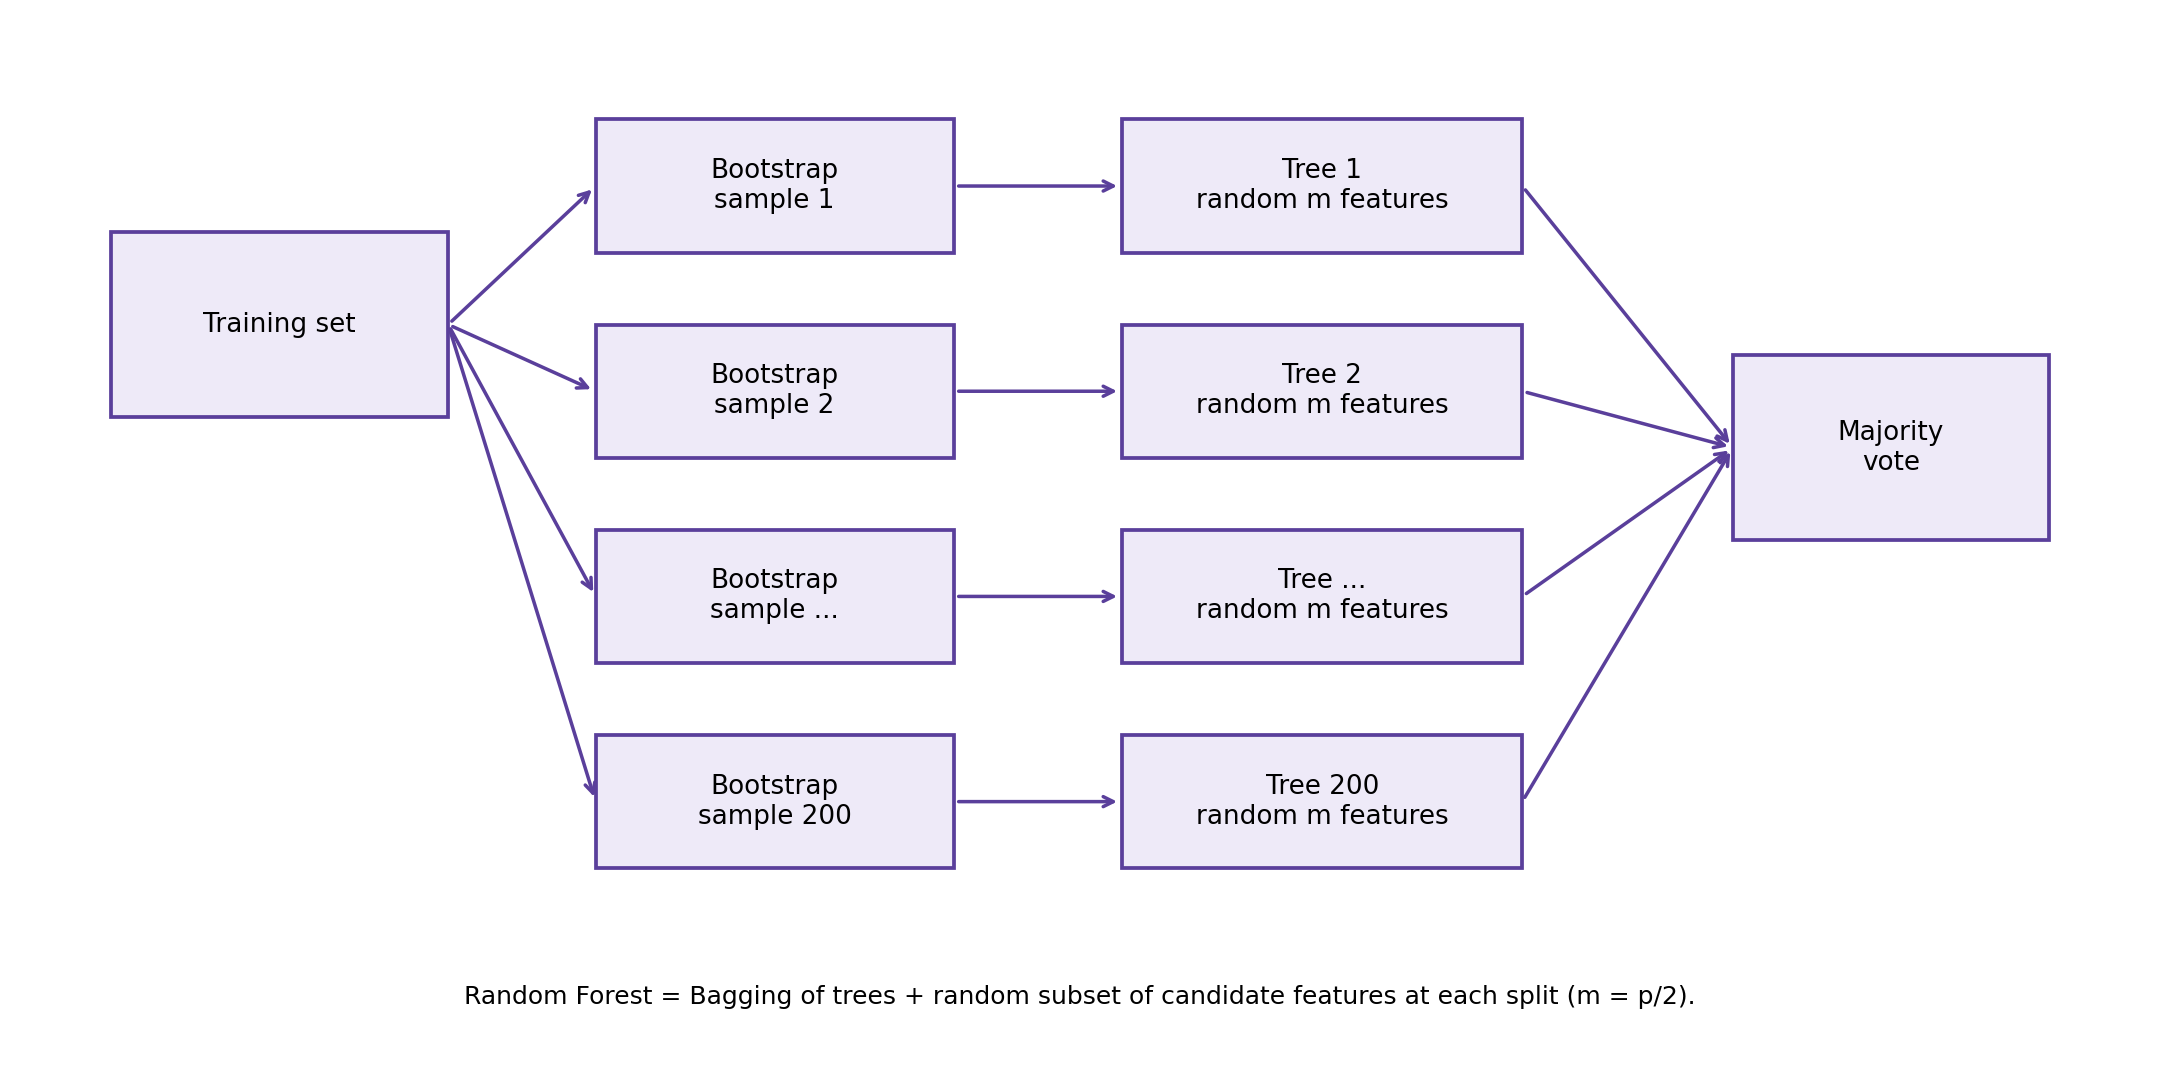
\includegraphics[width=0.92\textwidth]{q3_random_forest_concept.png}
\caption{Η βασική ιδέα του Random Forest.}
\end{figure}

\subsection{Τα δύο επίπεδα τυχαιότητας στο Random Forest}

Στο συγκεκριμένο μοντέλο υπάρχουν δύο διαφορετικά είδη τυχαιότητας.

\subsubsection{Πρώτο επίπεδο: τυχαίες γραμμές του training set}

Όπως και στο Bagging, κάθε δέντρο δεν εκπαιδεύεται ακριβώς στο ίδιο training
set. Για κάθε δέντρο φτιάχνεται ένα bootstrap δείγμα. Δηλαδή επιλέγονται
τυχαία \textbf{ολόκληρες γραμμές} από το training set, με επανάθεση.

Αυτό σημαίνει ότι μία γραμμή μπορεί να εμφανιστεί περισσότερες από μία φορές
στο bootstrap δείγμα, ενώ κάποια άλλη γραμμή μπορεί να μη χρησιμοποιηθεί
καθόλου από το συγκεκριμένο δέντρο.

Δεν παίρνουμε τυχαίες τιμές από κάθε στήλη ξεχωριστά. Παίρνουμε ολόκληρες
παρατηρήσεις κρασιών, ώστε να μη χαλάσει η σχέση που έχουν οι μεταβλητές
μεταξύ τους.

\subsubsection{Δεύτερο επίπεδο: τυχαίες μεταβλητές σε κάθε split}

Το δεύτερο επίπεδο τυχαιότητας είναι αυτό που κάνει το Random Forest να
διαφέρει από το απλό Bagging. Όταν ένα δέντρο βρίσκεται σε έναν κόμβο και θέλει
να αποφασίσει το επόμενο split, δεν επιτρέπεται να εξετάσει και τις 11
μεταβλητές. Εξετάζει μόνο $m=5$ τυχαία επιλεγμένες μεταβλητές.

Για παράδειγμα, σε έναν κόμβο μπορεί οι 5 υποψήφιες μεταβλητές να είναι:

\begin{center}
\code{chlorides}, \code{density}, \code{pH}, \code{alcohol}, \code{sulphates}.
\end{center}

Σε έναν άλλο κόμβο, ακόμα και μέσα στο ίδιο δέντρο, μπορεί οι 5 υποψήφιες
μεταβλητές να είναι διαφορετικές:

\begin{center}
\code{total sulfur dioxide}, \code{residual sugar}, \code{citric acid},
\code{free sulfur dioxide}, \code{fixed acidity}.
\end{center}

Αυτό γίνεται ξανά και ξανά, σε κάθε split και σε κάθε δέντρο.

\subsection{Τι σημαίνει \texorpdfstring{$m=p/2$}{m=p/2}}

Στο πρόβλημά μας οι προβλεπτικές μεταβλητές είναι:

\[
    p = 11.
\]

Οι 11 αυτές μεταβλητές είναι όλες οι μεταβλητές του dataset εκτός από:

\begin{itemize}
    \item τη \code{wine\_type}, γιατί αυτή είναι η μεταβλητή που θέλουμε να
    προβλέψουμε,
    \item την \code{quality}, γιατί η εκφώνηση λέει να μη χρησιμοποιηθεί.
\end{itemize}

Άρα οι predictors που χρησιμοποιούνται είναι:

\begin{center}
\begin{tabular}{lll}
\toprule
\code{fixed acidity} & \code{volatile acidity} & \code{citric acid} \\
\code{residual sugar} & \code{chlorides} & \code{free sulfur dioxide} \\
\code{total sulfur dioxide} & \code{density} & \code{pH} \\
\code{sulphates} & \code{alcohol} & \\
\bottomrule
\end{tabular}
\end{center}

Η εκφώνηση ζητά:

\[
    m = \frac{p}{2} = \frac{11}{2} = 5.5.
\]

Επειδή το \code{scikit-learn} χρειάζεται ακέραιο πλήθος χαρακτηριστικών όταν
δίνουμε το \code{max\_features} ως αριθμό, χρησιμοποιήθηκε:

\begin{center}
\code{max\_features = 5}.
\end{center}

Άρα, σε κάθε split, το Random Forest εξέταζε τυχαία 5 από τις 11 μεταβλητές.

Το σημαντικό είναι ότι το $m=5$ δεν σημαίνει ότι το μοντέλο χρησιμοποιεί μόνο 5
μεταβλητές συνολικά. Σημαίνει ότι \textbf{σε κάθε split} εξετάζει 5 τυχαίες
μεταβλητές. Σε άλλο split μπορεί να εξετάσει άλλες 5. Επομένως, συνολικά το
Random Forest μπορεί να αξιοποιήσει και τις 11 μεταβλητές, απλώς δεν τις
εξετάζει όλες ταυτόχρονα σε κάθε απόφαση.

\subsection{Πώς το λύσαμε}

Ο υπολογισμός του $m$ έγινε ως εξής:

\begin{lstlisting}[language=Python]
features = [col for col in df.columns if col not in ("quality", "wine_type")]
p = len(features)
max_features = p // 2
\end{lstlisting}

Το μοντέλο ορίστηκε ως:

\begin{lstlisting}[language=Python]
model = RandomForestClassifier(
    n_estimators=200,
    max_features=5,
    random_state=6931,
    n_jobs=-1,
)
\end{lstlisting}

Η διαδικασία εκπαίδευσης μπορεί να περιγραφεί βήμα-βήμα ως εξής:

\begin{enumerate}
    \item Κρατήσαμε ως predictors όλες τις μεταβλητές εκτός από
    \code{quality} και \code{wine\_type}.
    \item Χρησιμοποιήσαμε το ίδιο training set και test set με τα προηγούμενα
    ερωτήματα.
    \item Υπολογίσαμε ότι το πλήθος των predictors είναι $p=11$.
    \item Θέσαμε $m=p/2$, δηλαδή στην πράξη \code{max\_features=5}.
    \item Εκπαιδεύσαμε 200 δέντρα αποφάσεων.
    \item Κάθε δέντρο εκπαιδεύτηκε σε διαφορετικό bootstrap δείγμα του
    training set.
    \item Σε κάθε split κάθε δέντρου, εξετάστηκαν μόνο 5 τυχαίες μεταβλητές.
    \item Για κάθε παρατήρηση του test set, τα 200 δέντρα έδωσαν 200
    προβλέψεις.
    \item Η τελική πρόβλεψη ήταν η κλάση με τις περισσότερες ψήφους.
\end{enumerate}

Αν, για παράδειγμα, για ένα κρασί τα 200 δέντρα ψήφιζαν ως εξής:

\[
    184 \text{ δέντρα λένε white}
    \quad \text{και} \quad
    16 \text{ δέντρα λένε red},
\]

τότε το Random Forest θα προέβλεπε ότι το κρασί είναι \code{white}.

\subsection{Πώς παίρνει μία πρόβλεψη το Random Forest}

Για να γίνει πιο καθαρό, ας πάρουμε νοητά μία παρατήρηση από το test set, δηλαδή
ένα κρασί που το μοντέλο δεν έχει δει στην εκπαίδευση. Η παρατήρηση αυτή έχει
τιμές για τις 11 προβλεπτικές μεταβλητές.

Η παρατήρηση περνά από το πρώτο δέντρο και παίρνει μία πρόβλεψη. Μετά περνά από
το δεύτερο δέντρο και παίρνει άλλη μία πρόβλεψη. Αυτό συνεχίζεται μέχρι και το
δέντρο 200.

Στο τέλος μπορεί να έχουμε κάτι σαν:

\begin{center}
\begin{tabular}{lcc}
\toprule
 & \textbf{Ψήφοι για red} & \textbf{Ψήφοι για white} \\
\midrule
Παράδειγμα test κρασιού & 23 & 177 \\
\bottomrule
\end{tabular}
\end{center}

Επειδή οι περισσότερες ψήφοι είναι για \code{white}, η τελική πρόβλεψη είναι
\code{white}. Αυτός είναι ο λόγος που λέμε ότι το Random Forest είναι ensemble
μέθοδος: δεν εμπιστεύεται ένα μόνο μοντέλο, αλλά συνδυάζει πολλά μοντέλα.

\subsection{Αποτελέσματα}

\begin{table}[H]
\centering
\caption{Αποτελέσματα Random Forest.}
\begin{tabular}{lr}
\toprule
\textbf{Μέτρο} & \textbf{Τιμή} \\
\midrule
Πλήθος predictors $p$ & 11 \\
$p/2$ & 5.5 \\
Χρησιμοποιημένο \code{max\_features} & 5 \\
Test accuracy & 0.9666 \\
Test error & 0.0334 \\
Σωστές προβλέψεις & 1536 \\
Λανθασμένες προβλέψεις & 53 \\
\bottomrule
\end{tabular}
\end{table}

Ας διαβάσουμε τον πίνακα με απλά λόγια:

\begin{itemize}
    \item η ακρίβεια ήταν 0.9666, δηλαδή περίπου 96.66\%,
    \item το test error ήταν 0.0334, δηλαδή περίπου 3.34\%,
    \item από τις 1589 παρατηρήσεις του test set, οι 1536 ταξινομήθηκαν σωστά,
    \item οι 53 ταξινομήθηκαν λάθος.
\end{itemize}

Ο confusion matrix ήταν:

\begin{table}[H]
\centering
\caption{Confusion matrix για το Random Forest.}
\begin{tabular}{lcc}
\toprule
& \textbf{Πρόβλεψη red} & \textbf{Πρόβλεψη white} \\
\midrule
\textbf{Πραγματικό red} & 365 & 26 \\
\textbf{Πραγματικό white} & 27 & 1171 \\
\bottomrule
\end{tabular}
\end{table}

\begin{figure}[H]
\centering
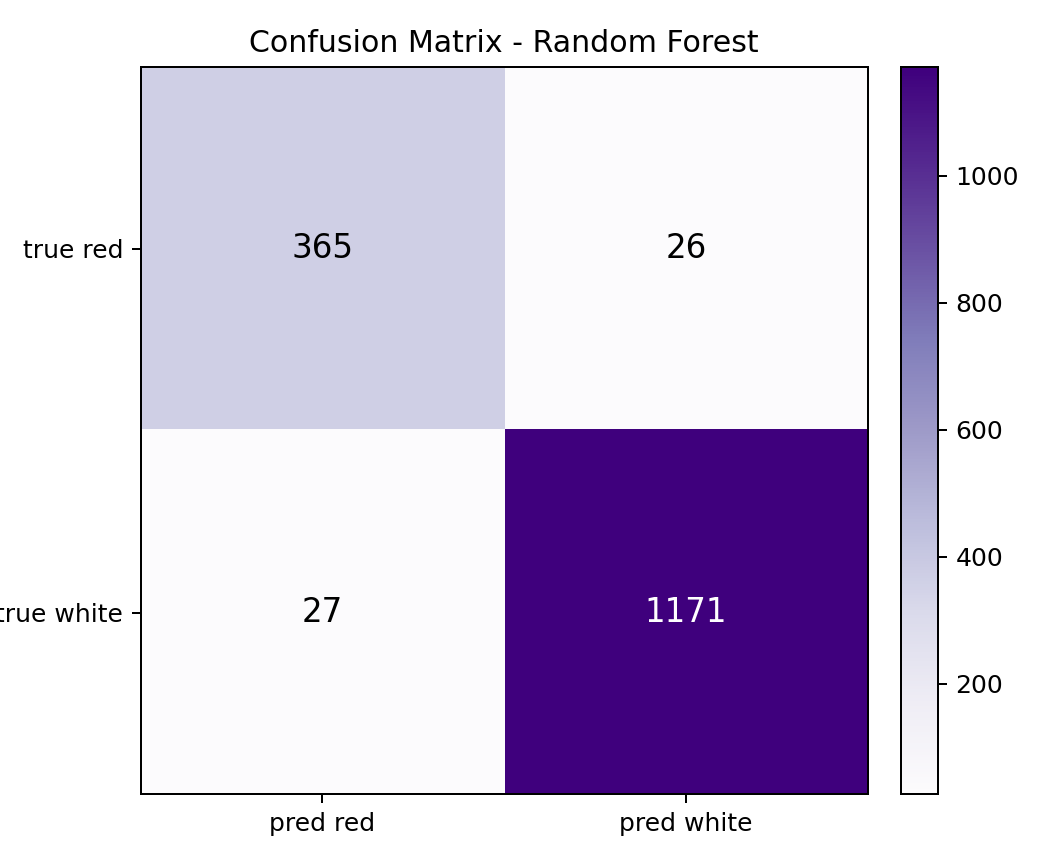
\includegraphics[width=0.62\textwidth]{q3_confusion_matrix.png}
\caption{Confusion matrix του Random Forest.}
\end{figure}

Ο confusion matrix μάς λέει πιο συγκεκριμένα πού έγιναν τα λάθη:

\begin{itemize}
    \item 365 κόκκινα κρασιά αναγνωρίστηκαν σωστά ως κόκκινα,
    \item 26 κόκκινα κρασιά προβλέφθηκαν λανθασμένα ως λευκά,
    \item 27 λευκά κρασιά προβλέφθηκαν λανθασμένα ως κόκκινα,
    \item 1171 λευκά κρασιά αναγνωρίστηκαν σωστά ως λευκά.
\end{itemize}

Άρα το μοντέλο κάνει λάθη και στις δύο κατευθύνσεις, αλλά τα λάθη είναι λίγα σε
σχέση με το συνολικό μέγεθος του test set.

\subsection{Σύγκριση με τα Ερωτήματα 1 και 2}

\begin{table}[H]
\centering
\caption{Σύγκριση των τριών πρώτων μοντέλων.}
\begin{tabular}{lrr}
\toprule
\textbf{Μοντέλο} & \textbf{Test Accuracy} & \textbf{Test Error} \\
\midrule
Decision Tree (\code{max\_depth=2}) & 0.9339 & 0.0661 \\
Bagging (200 estimators) & 0.9660 & 0.0340 \\
Random Forest (200 estimators, $m=5$) & 0.9666 & 0.0334 \\
\bottomrule
\end{tabular}
\end{table}

Το Random Forest έκανε 53 λάθη, δηλαδή ένα λιγότερο από το Bagging και 52
λιγότερα από το απλό δέντρο.

Η βελτίωση σε σχέση με το απλό δέντρο είναι μεγάλη. Αυτό είναι αναμενόμενο,
γιατί το απλό δέντρο του Ερωτήματος 1 είχε μέγιστο βάθος 2 και άρα ήταν πολύ
περιορισμένο. Μπορούσε να κάνει μόνο λίγα splits.

Η βελτίωση σε σχέση με το Bagging είναι πολύ μικρή. Αυτό δεν σημαίνει ότι το
Random Forest απέτυχε. Σημαίνει ότι, για το συγκεκριμένο dataset, το Bagging
ήταν ήδη πολύ δυνατό. Οι μεταβλητές \code{total sulfur dioxide} και
\code{chlorides} διαχωρίζουν αρκετά καλά τα κόκκινα από τα λευκά κρασιά, άρα
ακόμα και το Bagging έχει ήδη υψηλή ακρίβεια.

Το Random Forest κέρδισε οριακά επειδή μείωσε λίγο περισσότερο την ομοιότητα
ανάμεσα στα δέντρα. Όταν τα δέντρα είναι λιγότερο συσχετισμένα μεταξύ τους, τα
λάθη τους τείνουν να ακυρώνονται καλύτερα μέσω της ψηφοφορίας.

\subsection{Σημαντικότητα χαρακτηριστικών}

\begin{figure}[H]
\centering
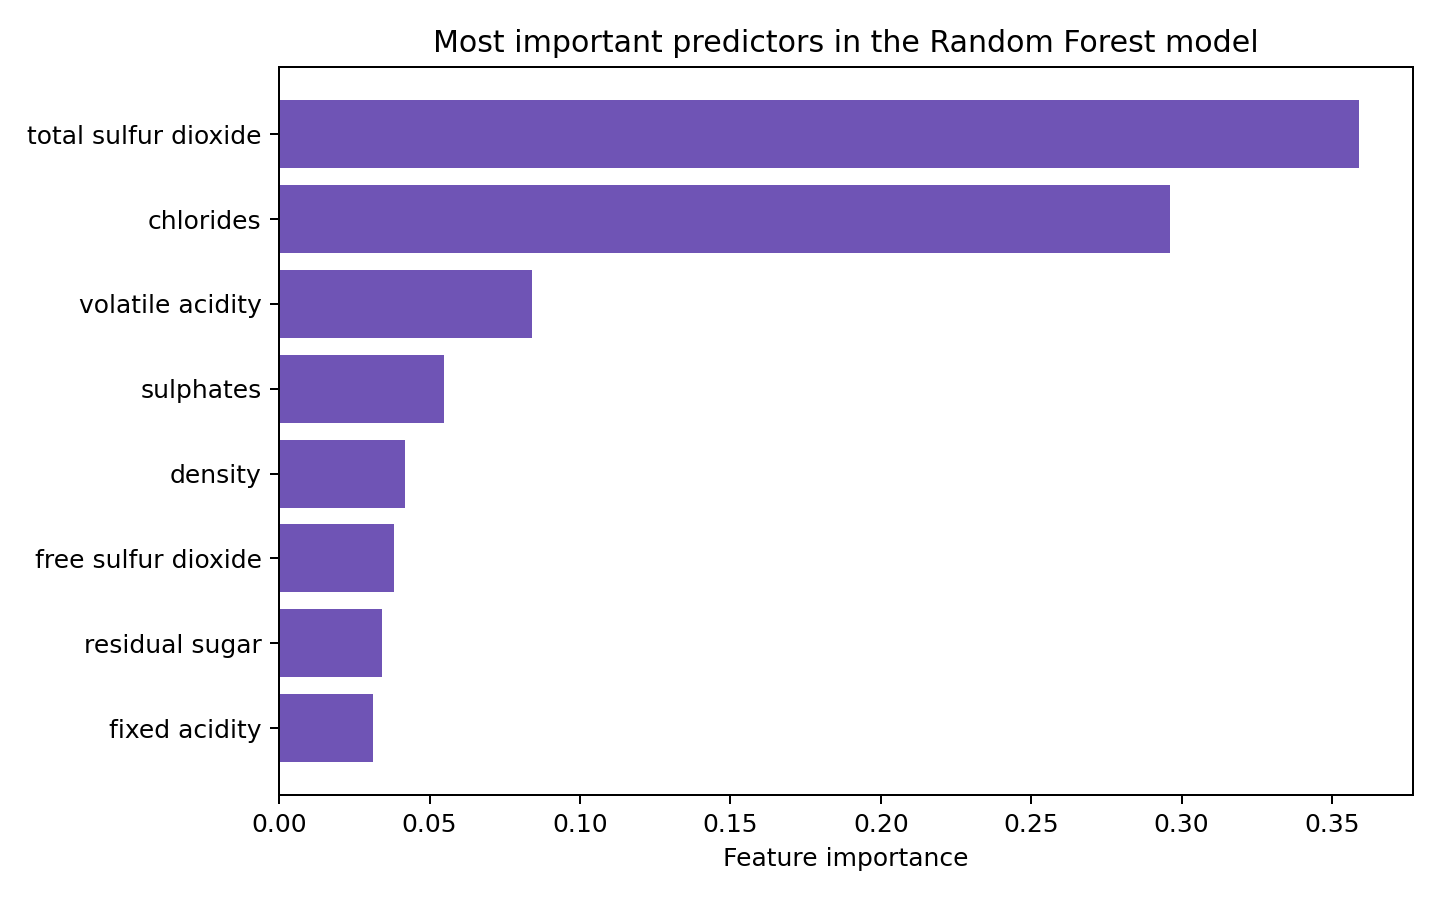
\includegraphics[width=0.82\textwidth]{q3_random_forest_feature_importance.png}
\caption{Οι σημαντικότερες μεταβλητές στο Random Forest.}
\end{figure}

Οι σημαντικότερες μεταβλητές ήταν και πάλι οι \code{total sulfur dioxide} και
\code{chlorides}. Αυτό είναι συνεπές με όσα είδαμε και στα δύο προηγούμενα
ερωτήματα.

Η σημαντικότητα χαρακτηριστικών στο Random Forest υπολογίζεται με βάση το πόσο
βοηθά κάθε μεταβλητή στη μείωση της ακαθαρσίας των κόμβων μέσα στα δέντρα.
Με πιο απλά λόγια, μία μεταβλητή θεωρείται σημαντική όταν χρησιμοποιείται συχνά
σε splits που κάνουν τους κόμβους πιο καθαρούς, δηλαδή όταν βοηθά να
ξεχωρίζουν καλύτερα τα κόκκινα από τα λευκά κρασιά.

Πρέπει όμως να το ερμηνεύουμε προσεκτικά. Η σημαντικότητα δεν σημαίνει ότι η
μεταβλητή είναι η αιτία που ένα κρασί είναι κόκκινο ή λευκό. Σημαίνει ότι,
μέσα στο συγκεκριμένο dataset και με το συγκεκριμένο μοντέλο, η μεταβλητή ήταν
χρήσιμη για την ταξινόμηση.

\subsection{Συμπέρασμα Ερωτήματος 3}

Το Random Forest με 200 δέντρα και \code{max\_features=5} πέτυχε test accuracy
0.9666. Η απόδοση ήταν πολύ καλύτερη από το απλό δέντρο και οριακά καλύτερη
από το Bagging. Η βελτίωση σε σχέση με το Bagging είναι μικρή, αλλά το Random
Forest παραμένει θεωρητικά πιο ισχυρή παραλλαγή, επειδή μειώνει τη συσχέτιση
μεταξύ των δέντρων μέσω της τυχαίας επιλογής χαρακτηριστικών.

Άρα, η βασική ιδέα που πρέπει να κρατήσουμε είναι η εξής: το Random Forest
βελτιώνει το Bagging όχι επειδή φτιάχνει απλώς περισσότερα δέντρα, αλλά επειδή
κάνει τα δέντρα πιο διαφορετικά μεταξύ τους. Αυτό το πετυχαίνει επιτρέποντας
σε κάθε split να δει μόνο ένα τυχαίο μέρος των διαθέσιμων μεταβλητών.

%=============================================================================
\section{Ερώτημα 4: Boosting με 200 επιμέρους μοντέλα}
%=============================================================================

\subsection{Τι ζητάει το ερώτημα}

Το τέταρτο ερώτημα είναι:

\begin{quote}
\textbf{«Να γίνει πρόβλεψη/εκτίμηση του τύπου κρασιού με τη μέθοδο Boosting,
χρησιμοποιώντας 200 επιμέρους μοντέλα, συντελεστή μάθησης 0.1 και μέγιστο
βάθος 1.»}
\end{quote}

Με απλά λόγια, θέλουμε ξανά να προβλέψουμε αν ένα κρασί είναι λευκό ή κόκκινο,
αλλά αυτή τη φορά με τη μέθοδο \textbf{Boosting}. Η βασική ιδέα του Boosting
είναι διαφορετική από το Bagging και το Random Forest. Στο Bagging και στο
Random Forest τα δέντρα μπορούν να εκπαιδευτούν σχετικά ανεξάρτητα μεταξύ
τους. Στο Boosting, όμως, τα μοντέλα χτίζονται \textbf{διαδοχικά}.

Αυτό είναι το πιο σημαντικό σημείο του ερωτήματος. Δεν φτιάχνουμε 200 δέντρα
που δουλεύουν ανεξάρτητα και μετά απλώς ψηφίζουν. Φτιάχνουμε 200 μικρά δέντρα
με σειρά. Το δεύτερο δέντρο εκπαιδεύεται αφού έχει ήδη φτιαχτεί το πρώτο, το
τρίτο αφού έχουν ήδη φτιαχτεί τα δύο πρώτα, και ούτω καθεξής. Κάθε νέο δέντρο
προσπαθεί να προσθέσει μία μικρή διόρθωση στο συνολικό μοντέλο.

Δηλαδή:

\begin{itemize}
    \item πρώτα εκπαιδεύεται ένα απλό μοντέλο,
    \item μετά εκπαιδεύεται ένα δεύτερο μοντέλο που προσπαθεί να διορθώσει τα
    λάθη του πρώτου,
    \item μετά ένα τρίτο που προσπαθεί να βελτιώσει ακόμη περισσότερο το
    σύνολο,
    \item και η διαδικασία συνεχίζεται μέχρι να φτάσουμε στα 200 μοντέλα.
\end{itemize}

Στο ερώτημα ζητούνται συγκεκριμένες τιμές:

\begin{center}
\code{n\_estimators = 200}, \hspace{0.7cm}
\code{learning\_rate = 0.1}, \hspace{0.7cm}
\code{max\_depth = 1}.
\end{center}

\subsection{Θεωρητικό υπόβαθρο}

Το Boosting είναι μία ensemble μέθοδος. Αυτό σημαίνει ότι δεν βασίζεται σε ένα
μόνο μοντέλο, αλλά συνδυάζει πολλά μικρότερα μοντέλα.

Η σημαντική διαφορά είναι ότι στο Boosting τα μοντέλα δεν φτιάχνονται όλα
ανεξάρτητα. Φτιάχνονται το ένα μετά το άλλο. Κάθε νέο μοντέλο προσπαθεί να
βελτιώσει το συνολικό μοντέλο που έχει δημιουργηθεί μέχρι εκείνη τη στιγμή.

Μπορούμε να το σκεφτούμε σαν μία επαναληπτική διαδικασία διόρθωσης:

\begin{enumerate}
    \item Το πρώτο μικρό δέντρο κάνει μία αρχική προσπάθεια ταξινόμησης.
    \item Το μοντέλο βλέπει σε ποιες παρατηρήσεις τα πήγε καλά και σε ποιες
    όχι.
    \item Το επόμενο μικρό δέντρο προσπαθεί να βοηθήσει κυρίως εκεί όπου το
    υπάρχον μοντέλο δυσκολεύτηκε.
    \item Η νέα γνώση προστίθεται στο συνολικό μοντέλο, αλλά με μικρό βάρος,
    επειδή έχουμε \code{learning\_rate=0.1}.
    \item Η διαδικασία επαναλαμβάνεται 200 φορές.
\end{enumerate}

Άρα το Boosting δεν λειτουργεί με τη λογική «πολλά ανεξάρτητα μοντέλα και
ψηφοφορία», όπως το Bagging και το Random Forest. Λειτουργεί με τη λογική
«χτίζω σταδιακά ένα δυνατό μοντέλο, προσθέτοντας κάθε φορά μία μικρή
διόρθωση».

\subsection{Η βασική διαφορά από Bagging και Random Forest}

Επειδή έχουμε ήδη δει Bagging και Random Forest, αξίζει να ξεκαθαρίσουμε τη
διαφορά τους από το Boosting.

\begin{table}[H]
\centering
\caption{Διαισθητική σύγκριση Bagging, Random Forest και Boosting.}
\begin{tabular}{p{0.25\textwidth}p{0.31\textwidth}p{0.31\textwidth}}
\toprule
\textbf{Μέθοδος} & \textbf{Πώς φτιάχνονται τα δέντρα} & \textbf{Κύρια ιδέα} \\
\midrule
Bagging &
Πολλά δέντρα φτιάχνονται σε διαφορετικά bootstrap δείγματα. &
Μειώνουμε την αστάθεια ενός δέντρου παίρνοντας μέσο όρο ή ψηφοφορία. \\
Random Forest &
Όπως το Bagging, αλλά σε κάθε split εξετάζεται τυχαίο υποσύνολο μεταβλητών. &
Κάνουμε τα δέντρα πιο διαφορετικά μεταξύ τους. \\
Boosting &
Τα δέντρα φτιάχνονται διαδοχικά, το ένα μετά το άλλο. &
Κάθε νέο δέντρο προσπαθεί να διορθώσει τις αδυναμίες του προηγούμενου συνόλου. \\
\bottomrule
\end{tabular}
\end{table}

Επομένως, το Boosting είναι πιο «καθοδηγούμενο». Δεν αφήνει απλώς τα δέντρα να
εκπαιδευτούν ανεξάρτητα. Κάθε νέο δέντρο εξαρτάται από το τι έχει ήδη μάθει το
μοντέλο μέχρι εκείνη τη στιγμή.

\subsection{Τι σημαίνει ότι το μοντέλο διορθώνει τα λάθη}

Η φράση «διορθώνει τα λάθη» είναι χρήσιμη, αλλά θέλει λίγη προσοχή. Δεν
σημαίνει ότι το δεύτερο δέντρο απλώς βρίσκει τις παρατηρήσεις που το πρώτο
δέντρο ταξινόμησε λάθος και τις απομνημονεύει.

Σημαίνει ότι το συνολικό μοντέλο κοιτάζει πού οι προβλέψεις του δεν είναι
αρκετά καλές και το επόμενο δέντρο προσπαθεί να προσθέσει πληροφορία προς τη
σωστή κατεύθυνση.

Στην ταξινόμηση κρασιού, το μοντέλο προσπαθεί να μάθει έναν τρόπο να δίνει
υψηλή πιθανότητα στην κλάση \code{white} όταν το κρασί είναι λευκό και υψηλή
πιθανότητα στην κλάση \code{red} όταν το κρασί είναι κόκκινο. Αν για κάποιο
λευκό κρασί το υπάρχον μοντέλο δεν είναι αρκετά σίγουρο ή γέρνει προς τη λάθος
κλάση, τα επόμενα δέντρα προσπαθούν να μετακινήσουν την πρόβλεψη προς τη σωστή
πλευρά.

Στο \code{GradientBoostingClassifier} αυτή η διόρθωση γίνεται με βάση την ιδέα
του \textbf{gradient}. Δεν χρειάζεται για την εργασία να μπούμε σε βαθιά
μαθηματικά, αλλά η διαίσθηση είναι η εξής:

\begin{quote}
Το μοντέλο κοιτάζει προς ποια κατεύθυνση πρέπει να αλλάξει τις προβλέψεις του
ώστε να μειωθεί το λάθος, και κάθε νέο μικρό δέντρο κάνει ένα μικρό βήμα προς
αυτή την κατεύθυνση.
\end{quote}

Γι' αυτό η μέθοδος λέγεται \textenglish{Gradient Boosting}.

\subsection{Τι είναι weak learner}

Στο Boosting συχνά χρησιμοποιούμε πολύ απλά μοντέλα, τα οποία λέγονται
\textbf{weak learners}. Ένας weak learner δεν είναι απαραίτητα πολύ ισχυρός
μόνος του. Μπορεί να κάνει αρκετά λάθη. Όμως, όταν συνδυάσουμε πολλούς weak
learners σωστά, μπορούμε να δημιουργήσουμε ένα πολύ ισχυρό μοντέλο.

Στο δικό μας ερώτημα, κάθε επιμέρους μοντέλο είναι δέντρο με:

\begin{center}
\code{max\_depth = 1}.
\end{center}

Ένα δέντρο βάθους 1 λέγεται συχνά \textenglish{decision stump}. Είναι ένα πολύ
απλό δέντρο, το οποίο κάνει μόνο έναν βασικό διαχωρισμό. Από μόνο του δεν έχει
μεγάλη εκφραστική δύναμη, αλλά πολλά τέτοια μικρά δέντρα μαζί μπορούν να
δώσουν πολύ καλή πρόβλεψη.

Για παράδειγμα, ένα τέτοιο δέντρο μπορεί να κάνει κάτι τόσο απλό όσο:

\begin{quote}
«Αν το \code{total sulfur dioxide} είναι πάνω από κάποιο όριο, τότε γέρνω προς
την κλάση \code{white}, αλλιώς γέρνω προς την κλάση \code{red}.»
\end{quote}

Ένα μόνο τέτοιο split δεν μπορεί να περιγράψει όλη την πολυπλοκότητα των
δεδομένων. Όμως το Boosting δεν βασίζεται σε ένα μόνο split. Προσθέτει 200
τέτοια μικρά κομμάτια πληροφορίας. Το καθένα είναι απλό, αλλά το άθροισμά τους
μπορεί να γίνει πολύ αποτελεσματικό.

\subsection{Γιατί χρησιμοποιούμε \texorpdfstring{\code{max\_depth=1}}{max\_depth=1}}

Η εκφώνηση ζητά το κάθε επιμέρους δέντρο να έχει μέγιστο βάθος 1. Αυτό σημαίνει
ότι κάθε δέντρο είναι πολύ απλό. Η επιλογή αυτή έχει νόημα στο Boosting για δύο
λόγους.

Πρώτον, αν κάθε επιμέρους δέντρο ήταν πολύ βαθύ, τότε κάθε δέντρο θα μπορούσε
να μάθει υπερβολικά πολλές λεπτομέρειες του training set. Αυτό θα αύξανε τον
κίνδυνο overfitting, δηλαδή το μοντέλο να τα πηγαίνει πολύ καλά στα δεδομένα
εκπαίδευσης αλλά όχι το ίδιο καλά σε νέα δεδομένα.

Δεύτερον, το Boosting θέλει συχνά πολλά μικρά και ελεγχόμενα βήματα. Ένα stump
είναι ένα μικρό βήμα. Δεν προσπαθεί να λύσει όλο το πρόβλημα μόνο του. Απλώς
προσθέτει μία μικρή διόρθωση στο συνολικό μοντέλο.

Άρα, το \code{max\_depth=1} κάνει κάθε επιμέρους μοντέλο απλό, αλλά επιτρέπει
στο σύνολο των 200 μοντέλων να γίνει ισχυρό.

\subsection{Τι σημαίνει learning rate}

Η παράμετρος \code{learning\_rate} ελέγχει πόσο έντονα επηρεάζει κάθε νέο
μοντέλο το συνολικό ensemble.

Στο ερώτημα χρησιμοποιούμε:

\begin{center}
\code{learning\_rate = 0.1}.
\end{center}

Αυτό σημαίνει ότι κάθε νέο δέντρο προστίθεται με σχετικά μικρό βάρος. Με απλά
λόγια, το μοντέλο μαθαίνει πιο αργά και πιο προσεκτικά. Ένα μικρό learning
rate μπορεί να βοηθήσει στη σταθερότητα της μεθόδου, επειδή αποφεύγει τις πολύ
απότομες αλλαγές από ένα μόνο επιμέρους μοντέλο.

Ένας πρακτικός τρόπος να το καταλάβουμε είναι ο εξής:

\begin{itemize}
    \item Αν το \code{learning\_rate} ήταν μεγάλο, κάθε νέο δέντρο θα άλλαζε
    έντονα το συνολικό μοντέλο.
    \item Αν το \code{learning\_rate} είναι μικρό, κάθε νέο δέντρο κάνει πιο
    προσεκτική διόρθωση.
\end{itemize}

Στο δικό μας μοντέλο το \code{learning\_rate=0.1} σημαίνει ότι κάθε δέντρο δεν
μπαίνει στο ensemble με πλήρη ένταση. Η συνεισφορά του μικραίνει. Έτσι το
μοντέλο χρειάζεται αρκετά δέντρα, εδώ 200, αλλά η εκπαίδευση γίνεται πιο
ομαλά.

\subsection{Η σχέση ανάμεσα σε \texorpdfstring{\code{n\_estimators}}{n\_estimators} και \texorpdfstring{\code{learning\_rate}}{learning\_rate}}

Οι δύο παράμετροι \code{n\_estimators} και \code{learning\_rate} πρέπει να
διαβάζονται μαζί.

\begin{itemize}
    \item Το \code{n\_estimators=200} λέει πόσα μικρά δέντρα θα προστεθούν.
    \item Το \code{learning\_rate=0.1} λέει πόσο δυνατά θα μετράει κάθε δέντρο.
\end{itemize}

Αν έχουμε μικρό learning rate, συνήθως χρειαζόμαστε περισσότερα δέντρα για να
μάθει αρκετά το μοντέλο. Αν έχουμε πολύ μεγάλο learning rate, μπορεί το μοντέλο
να μάθει γρήγορα, αλλά υπάρχει μεγαλύτερος κίνδυνος να κάνει απότομες και όχι
τόσο σταθερές διορθώσεις.

Στην εργασία, οι τιμές δεν επιλέγονται από εμάς ελεύθερα σε αυτό το ερώτημα.
Μας δίνονται από την εκφώνηση:

\begin{center}
\code{n\_estimators=200}, \quad
\code{learning\_rate=0.1}, \quad
\code{max\_depth=1}.
\end{center}

Άρα εδώ εφαρμόζουμε ακριβώς το μοντέλο που ζητάει η εκφώνηση. Η διερεύνηση
διαφορετικών τιμών θα γίνει αργότερα στο tuning.

\begin{figure}[H]
\centering
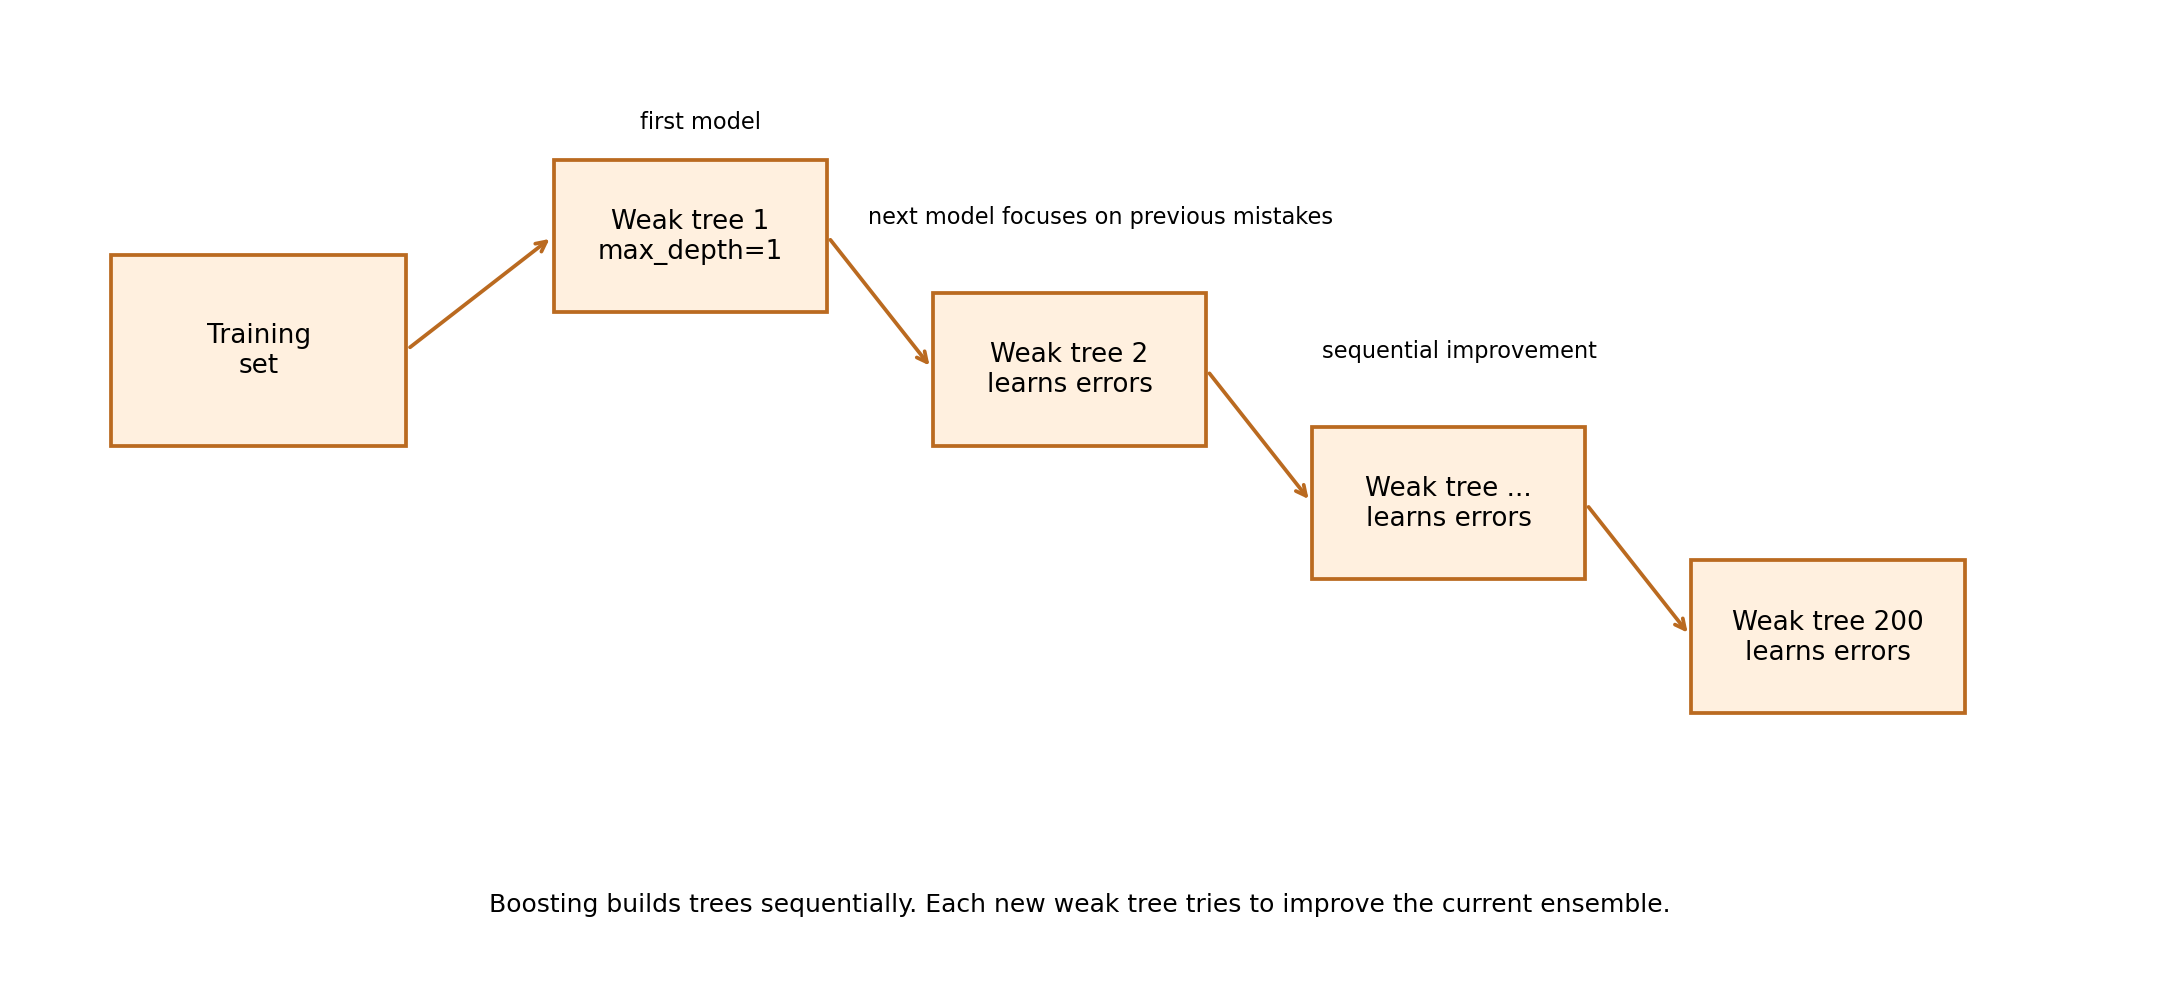
\includegraphics[width=0.92\textwidth]{q4_boosting_concept.png}
\caption{Η βασική ιδέα του Boosting: τα επιμέρους μοντέλα χτίζονται διαδοχικά.}
\end{figure}

\subsection{Πώς παίρνει τελική απόφαση το Boosting}

Στο Bagging και στο Random Forest λέγαμε ότι τα δέντρα ψηφίζουν. Στο Gradient
Boosting η εικόνα είναι λίγο διαφορετική. Τα μικρά δέντρα προσθέτουν
διαδοχικά διορθώσεις σε ένα συνολικό score.

Μπορούμε να το σκεφτούμε απλά ως εξής:

\begin{enumerate}
    \item Το μοντέλο ξεκινά με μία αρχική εκτίμηση.
    \item Το πρώτο μικρό δέντρο προσθέτει μία μικρή διόρθωση.
    \item Το δεύτερο μικρό δέντρο προσθέτει άλλη μία μικρή διόρθωση.
    \item Μετά από 200 τέτοιες διορθώσεις, το μοντέλο έχει ένα τελικό score.
    \item Το score μετατρέπεται σε πρόβλεψη κλάσης, δηλαδή \code{red} ή
    \code{white}.
\end{enumerate}

Άρα δεν είναι απλώς «200 ψήφοι». Είναι περισσότερο σαν άθροισμα πολλών μικρών
διορθώσεων. Αυτή είναι η βασική λογική του Gradient Boosting.

\subsection{Πώς το λύσαμε}

Χρησιμοποιήσαμε το ίδιο dataset, τους ίδιους predictors και το ίδιο train/test
split με τα προηγούμενα ερωτήματα. Η μεταβλητή στόχος ήταν πάλι η
\code{wine\_type}, με κωδικοποίηση \code{red=0} και \code{white=1}.

Το μοντέλο ορίστηκε ως:

\begin{lstlisting}[language=Python]
model = GradientBoostingClassifier(
    n_estimators=200,
    learning_rate=0.1,
    max_depth=1,
    random_state=6931,
)
\end{lstlisting}

Ας δούμε τι σημαίνει κάθε παράμετρος:

\begin{itemize}
    \item \code{GradientBoostingClassifier}: δηλώνει ότι χρησιμοποιούμε
    Boosting για ταξινόμηση.
    \item \code{n\_estimators=200}: το μοντέλο θα αποτελείται από 200
    επιμέρους δέντρα.
    \item \code{learning\_rate=0.1}: κάθε νέο δέντρο επηρεάζει το συνολικό
    μοντέλο με σχετικά μικρό βήμα.
    \item \code{max\_depth=1}: κάθε επιμέρους δέντρο είναι πολύ απλό.
    \item \code{random\_state=6931}: τα αποτελέσματα είναι αναπαραγώγιμα.
\end{itemize}

Η συνολική μεθοδολογία ήταν:

\begin{enumerate}
    \item Φορτώσαμε τα δεδομένα κρασιού.
    \item Αφαιρέσαμε τη μεταβλητή \code{quality}, επειδή η εκφώνηση λέει να μη
    χρησιμοποιηθεί ως predictor.
    \item Ορίσαμε ως στόχο τη μεταβλητή \code{wine\_type}.
    \item Χωρίσαμε τα δεδομένα σε training set 70\% και test set 30\%, όπως και
    στα προηγούμενα ερωτήματα.
    \item Εκπαιδεύσαμε το \code{GradientBoostingClassifier} μόνο στο training
    set.
    \item Χρησιμοποιήσαμε το εκπαιδευμένο μοντέλο για να προβλέψουμε τις
    κλάσεις των παρατηρήσεων του test set.
    \item Συγκρίναμε τις προβλέψεις με τις πραγματικές τιμές του test set.
    \item Υπολογίσαμε το test accuracy, το test error και τον confusion matrix.
\end{enumerate}

Είναι σημαντικό ότι το test set δεν χρησιμοποιείται για την εκπαίδευση. Το
κρατάμε μόνο για την τελική αξιολόγηση, ώστε να δούμε πώς συμπεριφέρεται το
μοντέλο σε δεδομένα που δεν έχει δει.

Μετά την εκπαίδευση, έγιναν προβλέψεις στο test set:

\begin{lstlisting}[language=Python]
y_pred = model.predict(X_test)
\end{lstlisting}

και υπολογίστηκαν:

\begin{lstlisting}[language=Python]
accuracy = accuracy_score(y_test, y_pred)
test_error = 1 - accuracy
\end{lstlisting}

\subsection{Αποτελέσματα}

\begin{table}[H]
\centering
\caption{Αποτελέσματα Boosting.}
\begin{tabular}{lr}
\toprule
\textbf{Μέτρο} & \textbf{Τιμή} \\
\midrule
\code{n\_estimators} & 200 \\
\code{learning\_rate} & 0.1 \\
\code{max\_depth} & 1 \\
Test accuracy & 0.9679 \\
Test error & 0.0321 \\
Σωστές προβλέψεις & 1538 \\
Λανθασμένες προβλέψεις & 51 \\
\bottomrule
\end{tabular}
\end{table}

Το Boosting πέτυχε:

\begin{center}
\textbf{Test accuracy = 0.9679}
\end{center}

δηλαδή ταξινόμησε σωστά περίπου το 96.79\% των test παρατηρήσεων.

Αν το γράψουμε ως ποσοστά:

\[
    0.9679 \times 100 = 96.79\%.
\]

Το αντίστοιχο test error είναι:

\[
    1 - 0.9679 = 0.0321,
\]

δηλαδή περίπου:

\[
    0.0321 \times 100 = 3.21\%.
\]

Άρα, σε απλή γλώσσα, το μοντέλο κάνει λάθος περίπου σε 3 από τις 100
παρατηρήσεις του test set.

\subsection{Confusion matrix}

Ο confusion matrix ήταν:

\begin{table}[H]
\centering
\caption{Confusion matrix για το Boosting.}
\begin{tabular}{lcc}
\toprule
& \textbf{Πρόβλεψη red} & \textbf{Πρόβλεψη white} \\
\midrule
\textbf{Πραγματικό red} & 361 & 30 \\
\textbf{Πραγματικό white} & 21 & 1177 \\
\bottomrule
\end{tabular}
\end{table}

\begin{figure}[H]
\centering
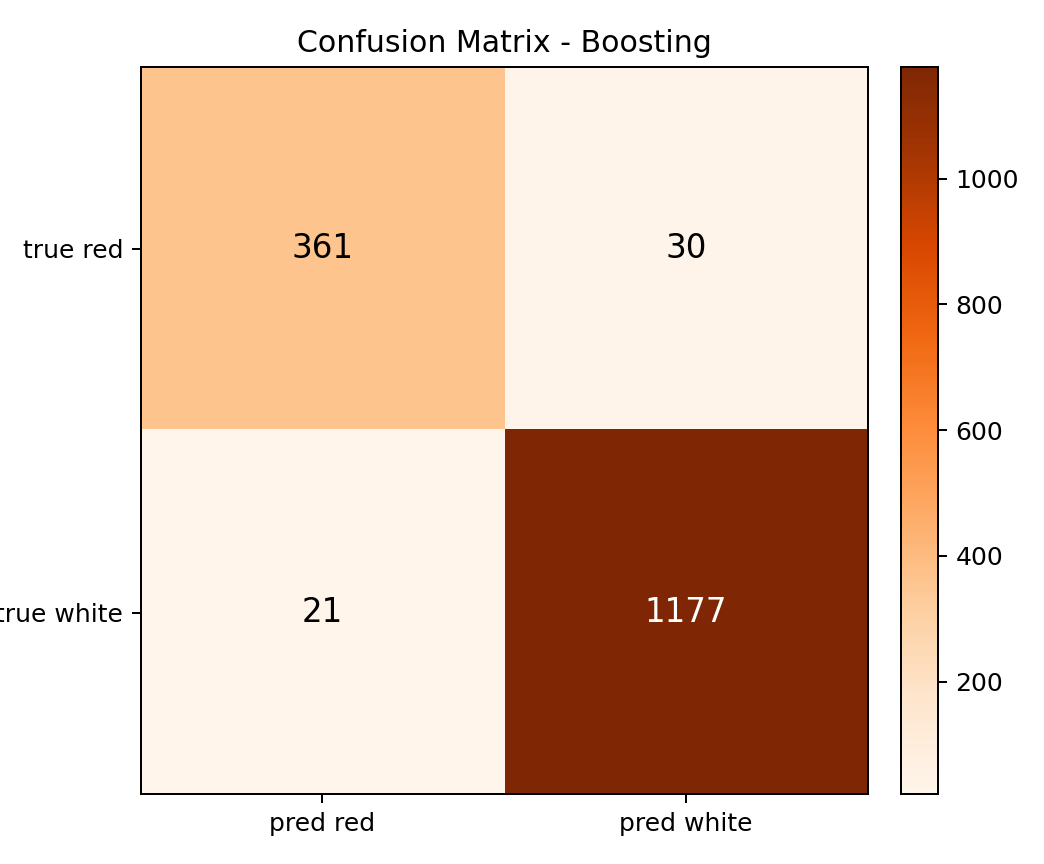
\includegraphics[width=0.62\textwidth]{q4_confusion_matrix.png}
\caption{Confusion matrix του Boosting.}
\end{figure}

Ο πίνακας δείχνει ότι:

\begin{itemize}
    \item 361 κόκκινα κρασιά ταξινομήθηκαν σωστά ως κόκκινα,
    \item 30 κόκκινα κρασιά ταξινομήθηκαν λάθος ως λευκά,
    \item 21 λευκά κρασιά ταξινομήθηκαν λάθος ως κόκκινα,
    \item 1177 λευκά κρασιά ταξινομήθηκαν σωστά ως λευκά.
\end{itemize}

Άρα οι σωστές προβλέψεις είναι:

\[
    361 + 1177 = 1538.
\]

Τα συνολικά λάθη είναι:

\[
    30 + 21 = 51.
\]

Παρατηρούμε επίσης ότι το μοντέλο έκανε:

\begin{itemize}
    \item 30 λάθη όπου κόκκινα κρασιά προβλέφθηκαν ως λευκά,
    \item 21 λάθη όπου λευκά κρασιά προβλέφθηκαν ως κόκκινα.
\end{itemize}

Δηλαδή, στο συγκεκριμένο test set, το Boosting μπέρδεψε λίγο περισσότερα
κόκκινα κρασιά προς την κατεύθυνση του λευκού από ό,τι λευκά προς την
κατεύθυνση του κόκκινου. Παρ' όλα αυτά, το συνολικό πλήθος λαθών είναι πολύ
μικρό.

\subsection{Σύγκριση με τα προηγούμενα μοντέλα}

\begin{table}[H]
\centering
\caption{Σύγκριση των τεσσάρων πρώτων μοντέλων.}
\begin{tabular}{lrr}
\toprule
\textbf{Μοντέλο} & \textbf{Test Accuracy} & \textbf{Test Error} \\
\midrule
Decision Tree (\code{max\_depth=2}) & 0.9339 & 0.0661 \\
Bagging (200 estimators) & 0.9660 & 0.0340 \\
Random Forest (200 estimators, $m=5$) & 0.9666 & 0.0334 \\
Boosting (200 estimators) & 0.9679 & 0.0321 \\
\bottomrule
\end{tabular}
\end{table}

Μέχρι τώρα, το Boosting έχει την καλύτερη test accuracy. Η διαφορά από το
Random Forest είναι μικρή, αλλά το Boosting έκανε τα λιγότερα συνολικά λάθη:

\begin{center}
\begin{tabular}{lrr}
\toprule
\textbf{Μοντέλο} & \textbf{Λάθη} & \textbf{Σωστές προβλέψεις} \\
\midrule
Decision Tree & 105 & 1484 \\
Bagging & 54 & 1535 \\
Random Forest & 53 & 1536 \\
Boosting & 51 & 1538 \\
\bottomrule
\end{tabular}
\end{center}

Η διαφορά ανάμεσα σε Bagging, Random Forest και Boosting δεν είναι τεράστια,
επειδή και οι τρεις ensemble μέθοδοι δουλεύουν πολύ καλά στο συγκεκριμένο
πρόβλημα. Όμως το Boosting έχει το μικρότερο test error από τα αρχικά μοντέλα:

\[
    0.0321 < 0.0334 < 0.0340 < 0.0661.
\]

Αυτό σημαίνει ότι, στο συγκεκριμένο train/test split, το Boosting ήταν το πιο
ακριβές από τα τέσσερα πρώτα μοντέλα.

Η βελτίωση σε σχέση με το Random Forest είναι μικρή:

\[
    0.9679 - 0.9666 = 0.0013.
\]

Σε ποσοστιαίες μονάδες, αυτό είναι περίπου 0.13 ποσοστιαίες μονάδες. Άρα δεν
λέμε ότι το Boosting είναι εντυπωσιακά καλύτερο από το Random Forest. Λέμε ότι
ήταν οριακά καλύτερο στα συγκεκριμένα test δεδομένα.

\subsection{Σημαντικότητα χαρακτηριστικών}

Το Boosting δίνει επίσης μία ένδειξη για το ποιες μεταβλητές βοήθησαν
περισσότερο στην ταξινόμηση.

\begin{figure}[H]
\centering
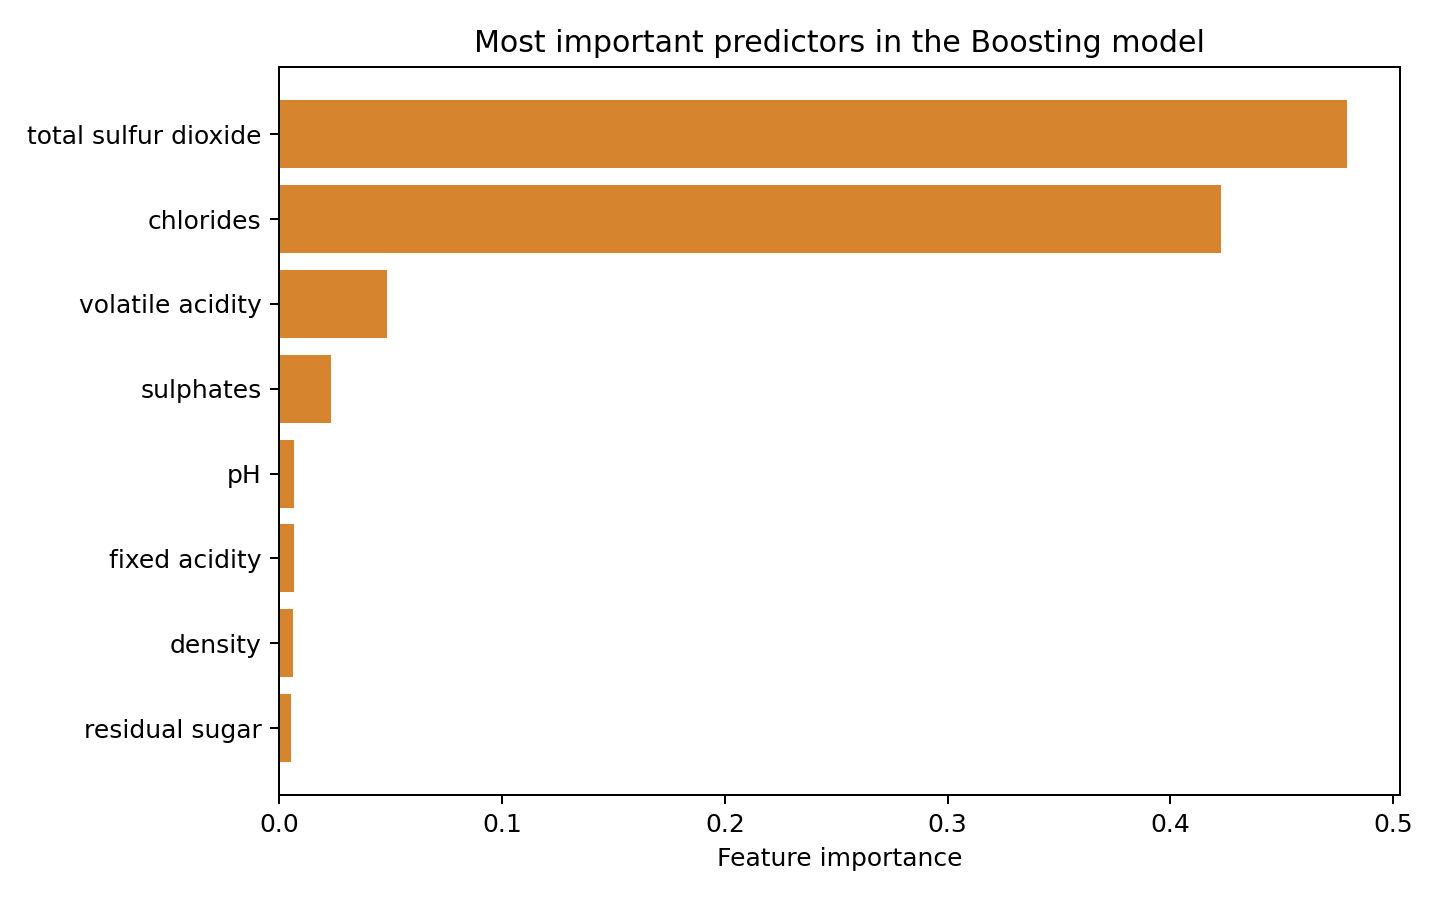
\includegraphics[width=0.82\textwidth]{q4_boosting_feature_importance.png}
\caption{Οι σημαντικότερες μεταβλητές στο Boosting.}
\end{figure}

Οι δύο σημαντικότερες μεταβλητές ήταν και εδώ οι:

\begin{itemize}
    \item \code{total sulfur dioxide}
    \item \code{chlorides}
\end{itemize}

Αυτό επιβεβαιώνει για ακόμη μία φορά ότι αυτές οι μεταβλητές είναι πολύ
χρήσιμες για τη διάκριση λευκού και κόκκινου κρασιού.

Η ερμηνεία εδώ είναι παρόμοια με τα προηγούμενα δέντρα, αλλά χρειάζεται λίγη
προσοχή. Η σημαντικότητα χαρακτηριστικών στο Boosting προκύπτει από το πόσο
συχνά και πόσο αποτελεσματικά χρησιμοποιείται μία μεταβλητή στα μικρά δέντρα
για να μειώσει το λάθος του μοντέλου.

Επειδή κάθε stump έχει μόνο ένα split, κάθε μικρό δέντρο μπορεί να βασιστεί σε
μία βασική μεταβλητή κάθε φορά. Αν μία μεταβλητή εμφανίζεται συχνά σε χρήσιμα
splits, τότε αποκτά μεγαλύτερη σημαντικότητα.

Το ότι οι \code{total sulfur dioxide} και \code{chlorides} παραμένουν
σημαντικές και στο Boosting είναι σημαντικό εύρημα, γιατί βλέπουμε συνέπεια
ανάμεσα σε διαφορετικές μεθόδους:

\begin{itemize}
    \item το απλό δέντρο τις χρησιμοποίησε στους βασικούς διαχωρισμούς,
    \item το Bagging τις ανέδειξε ως ισχυρές μεταβλητές,
    \item το Random Forest τις ανέδειξε ξανά,
    \item και το Boosting δείχνει ότι βοηθούν και στη διαδοχική διόρθωση των
    προβλέψεων.
\end{itemize}

\subsection{Συμπέρασμα Ερωτήματος 4}

Το Boosting με 200 επιμέρους μοντέλα, \code{learning\_rate=0.1} και
\code{max\_depth=1} πέτυχε test accuracy 0.9679. Είναι το καλύτερο αποτέλεσμα
μέχρι στιγμής ανάμεσα στα αρχικά μοντέλα των Ερωτημάτων 1--4.

Η μέθοδος πέτυχε υψηλή απόδοση παρότι κάθε επιμέρους δέντρο ήταν πολύ απλό.
Αυτό δείχνει τη δύναμη του Boosting: πολλά απλά μοντέλα, όταν συνδυαστούν
διαδοχικά και σωστά, μπορούν να δημιουργήσουν έναν πολύ ισχυρό ταξινομητή.

Το βασικό συμπέρασμα είναι ότι το Boosting λειτουργεί καλά επειδή μαθαίνει
σταδιακά. Δεν προσπαθεί να φτιάξει ένα πολύ περίπλοκο δέντρο από την αρχή.
Αντίθετα, φτιάχνει πολλά απλά δέντρα, όπου το καθένα διορθώνει λίγο το
συνολικό μοντέλο. Με \code{learning\_rate=0.1}, αυτές οι διορθώσεις είναι
προσεκτικές, και με \code{n\_estimators=200} υπάρχουν αρκετά βήματα ώστε το
μοντέλο να γίνει πολύ ακριβές.

%=============================================================================
\section{Ερώτημα 5: Test error του δέντρου συναρτήσει του βάθους}
%=============================================================================

\subsection{Τι ζητάει το ερώτημα}

Το πέμπτο ερώτημα είναι:

\begin{quote}
\textbf{«Να παρασταθεί γραφικά το test error της μεθόδου του ερωτήματος 1
συναρτήσει του βάθους του δέντρου. Τι παρατηρείτε; Σχολιάστε.»}
\end{quote}

Με απλά λόγια, μέχρι τώρα στο Ερώτημα 1 χρησιμοποιήσαμε ένα δέντρο με
\code{max\_depth=2}. Τώρα η εκφώνηση μάς ζητά να μην κρατήσουμε σταθερό το
βάθος, αλλά να δοκιμάσουμε πολλά διαφορετικά βάθη και να δούμε πώς αλλάζει το
test error.

Το ερώτημα θέλει να απαντήσουμε σε κάτι πολύ σημαντικό:

\begin{quote}
Αν κάνουμε το δέντρο πιο βαθύ, γίνεται πάντα καλύτερο;
\end{quote}

Η απάντηση, όπως θα δούμε, είναι όχι. Μέχρι ένα σημείο το μεγαλύτερο βάθος
βοηθά. Μετά από ένα σημείο, όμως, το δέντρο γίνεται υπερβολικά σύνθετο και
μπορεί να αρχίσει να γενικεύει χειρότερα.

\subsection{Θεωρητικό υπόβαθρο}

Το βάθος ενός δέντρου καθορίζει πόσο σύνθετο μπορεί να γίνει το μοντέλο.

\begin{itemize}
    \item Ένα πολύ ρηχό δέντρο έχει λίγους κανόνες και είναι πολύ απλό.
    \item Ένα πολύ βαθύ δέντρο έχει πολλούς κανόνες και μπορεί να ξεχωρίσει
    λεπτομέρειες στα δεδομένα.
\end{itemize}

Αν το δέντρο είναι υπερβολικά απλό, μπορεί να μην καταλαβαίνει αρκετά καλά τη
σχέση ανάμεσα στα χαρακτηριστικά και στον τύπο κρασιού. Αυτό λέγεται
\textbf{underfitting}.

Αν το δέντρο είναι υπερβολικά βαθύ, μπορεί να αρχίσει να μαθαίνει όχι μόνο το
γενικό μοτίβο, αλλά και τυχαίες λεπτομέρειες του training set. Αυτό λέγεται
\textbf{overfitting}.

\begin{figure}[H]
\centering
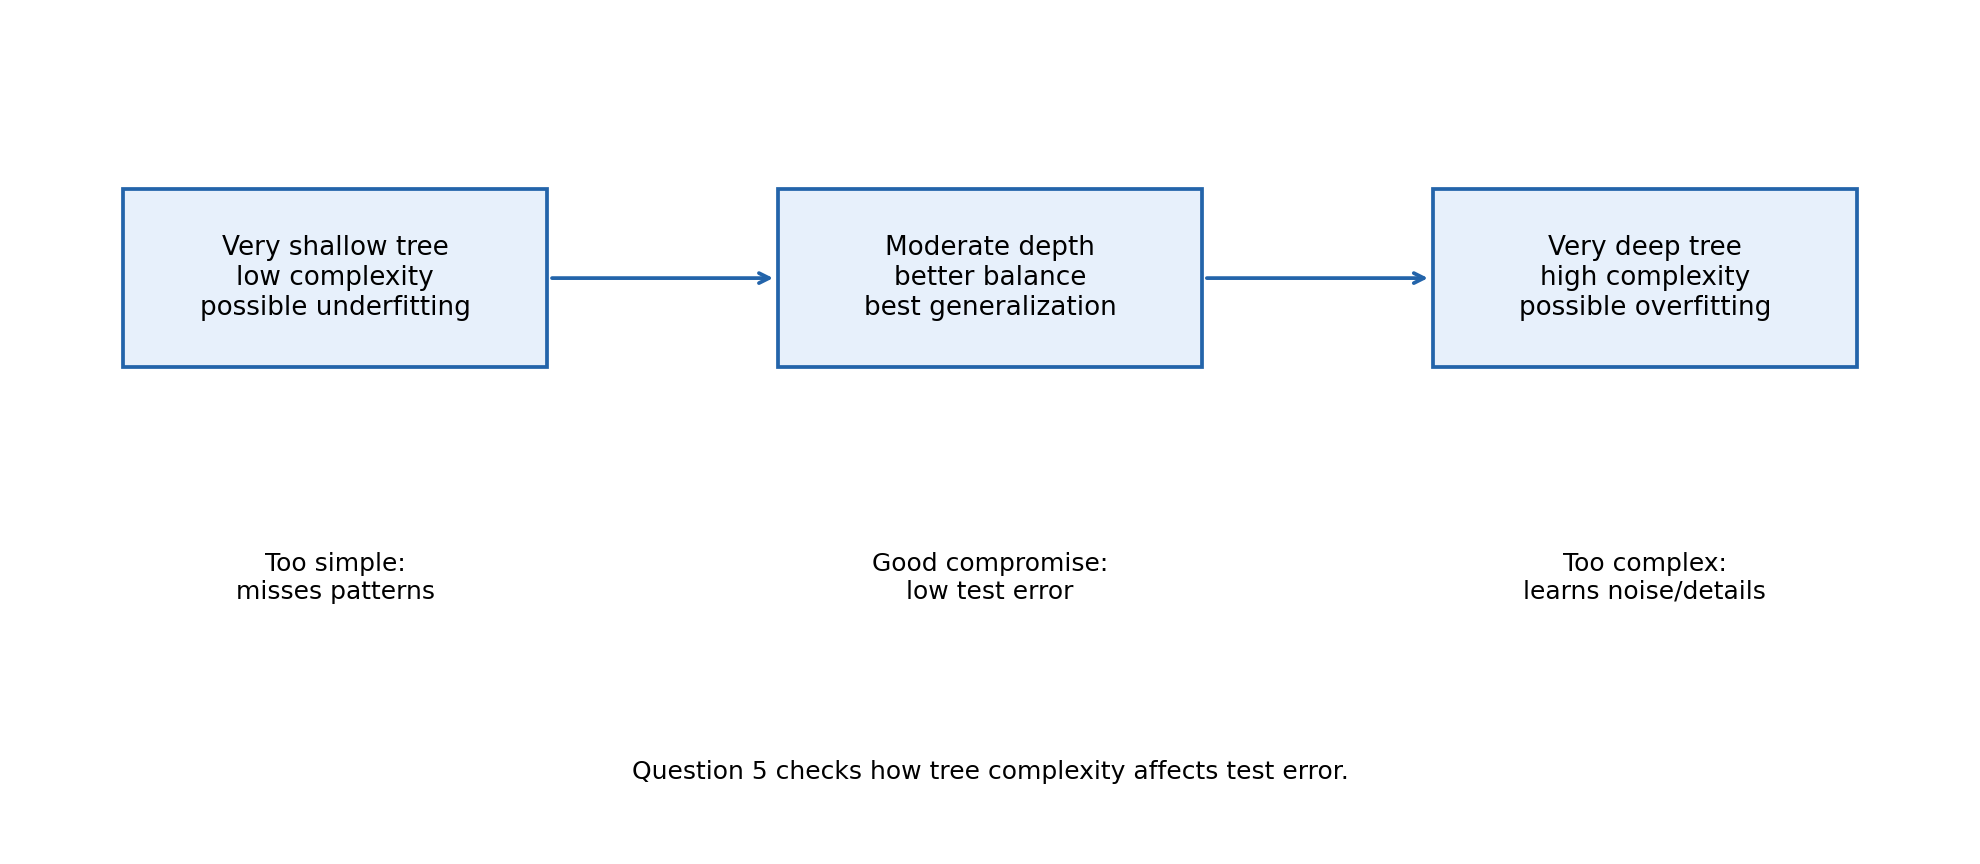
\includegraphics[width=0.88\textwidth]{q5_tree_depth_concept.png}
\caption{Η βασική ιδέα του Ερωτήματος 5: πολύ μικρό, μέτριο και πολύ μεγάλο βάθος.}
\end{figure}

\subsection{Τι είναι test error}

Το test error είναι:

\[
    \text{Test Error} = 1 - \text{Test Accuracy}.
\]

Αν ένα μοντέλο έχει test accuracy 0.9339, τότε:

\[
    \text{Test Error} = 1 - 0.9339 = 0.0661.
\]

Το test error δείχνει το ποσοστό των test παρατηρήσεων που ταξινομήθηκαν
λάθος. Όσο μικρότερο είναι, τόσο καλύτερο είναι το μοντέλο.

\subsection{Πώς το λύσαμε}

Χρησιμοποιήσαμε το ίδιο dataset και το ίδιο train/test split με τα προηγούμενα
ερωτήματα. Στη συνέχεια εκπαιδεύσαμε πολλά δέντρα ταξινόμησης, αλλάζοντας την
τιμή του \code{max\_depth}.

Δοκιμάσαμε βάθη:

\begin{center}
\code{max\_depth = 1, 2, 3, ..., 20}.
\end{center}

Για κάθε βάθος εκπαιδεύτηκε ξεχωριστό δέντρο και υπολογίστηκε το test error:

\begin{lstlisting}[language=Python]
for depth in range(1, 21):
    model = DecisionTreeClassifier(max_depth=depth, random_state=6931)
    model.fit(X_train, y_train)
    y_pred = model.predict(X_test)
    accuracy = accuracy_score(y_test, y_pred)
    test_error = 1 - accuracy
\end{lstlisting}

Έτσι πήραμε έναν πίνακα που δείχνει πώς αλλάζει το test error ανάλογα με το
βάθος του δέντρου.

\subsection{Αριθμητικά αποτελέσματα}

\begin{table}[H]
\centering
\caption{Test accuracy και test error για διαφορετικά βάθη δέντρου.}
\small
\begin{tabular}{rrr|rrr}
\toprule
\textbf{Depth} & \textbf{Accuracy} & \textbf{Error} &
\textbf{Depth} & \textbf{Accuracy} & \textbf{Error} \\
\midrule
1  & 0.9119 & 0.0881 & 11 & 0.9610 & 0.0390 \\
2  & 0.9339 & 0.0661 & 12 & 0.9497 & 0.0503 \\
3  & 0.9509 & 0.0491 & 13 & 0.9497 & 0.0503 \\
4  & 0.9629 & 0.0371 & 14 & 0.9484 & 0.0516 \\
5  & 0.9641 & 0.0359 & 15 & 0.9465 & 0.0535 \\
6  & 0.9654 & 0.0346 & 16 & 0.9396 & 0.0604 \\
7  & 0.9616 & 0.0384 & 17 & 0.9408 & 0.0592 \\
8  & 0.9616 & 0.0384 & 18 & 0.9415 & 0.0585 \\
9  & 0.9604 & 0.0396 & 19 & 0.9358 & 0.0642 \\
10 & 0.9597 & 0.0403 & 20 & 0.9346 & 0.0654 \\
\bottomrule
\end{tabular}
\end{table}

\begin{figure}[H]
\centering
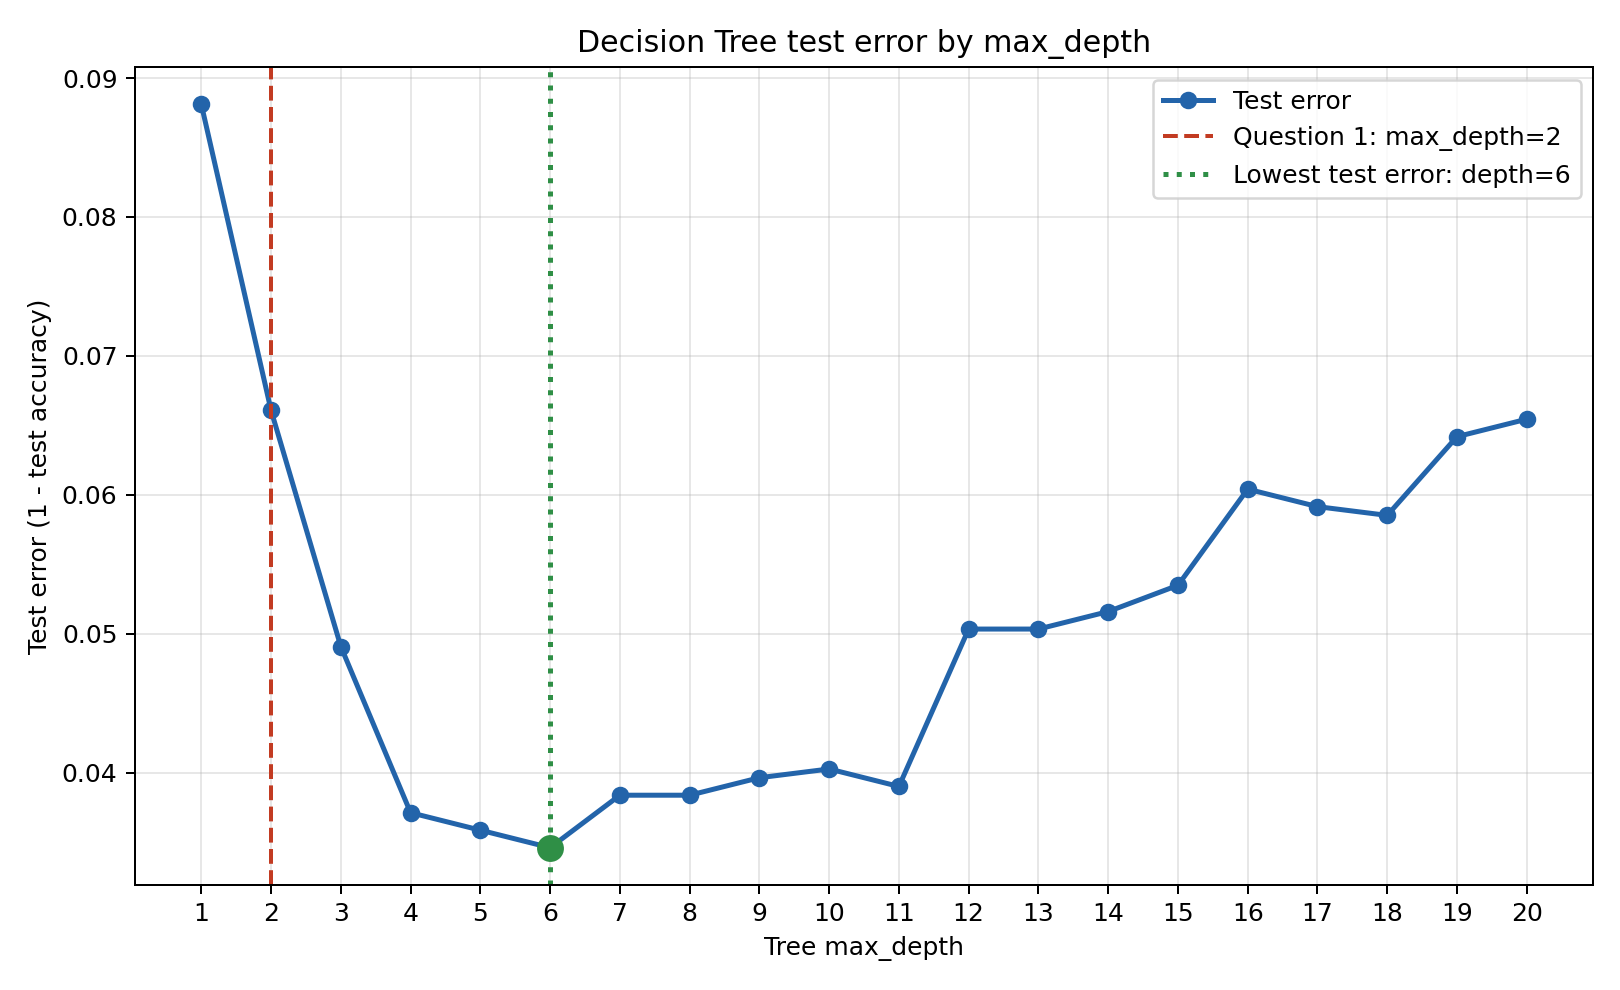
\includegraphics[width=0.88\textwidth]{q5_tree_depth_error.png}
\caption{Test error του δέντρου ταξινόμησης συναρτήσει του \code{max\_depth}.}
\end{figure}

\subsection{Τι παρατηρούμε}

Στα πολύ μικρά βάθη, το test error είναι σχετικά υψηλό. Για παράδειγμα:

\begin{itemize}
    \item για \code{max\_depth=1}, το test error είναι 0.0881,
    \item για \code{max\_depth=2}, το test error είναι 0.0661.
\end{itemize}

Αυτό σημαίνει ότι ένα πολύ απλό δέντρο δεν αρκεί για να αποτυπώσει πλήρως τη
δομή των δεδομένων. Έχει λίγους κανόνες και άρα δεν μπορεί να διαχωρίσει
τέλεια τα λευκά από τα κόκκινα κρασιά.

Καθώς αυξάνεται το βάθος, το test error μειώνεται. Η καλύτερη τιμή εμφανίζεται
στο:

\begin{center}
\code{max\_depth = 6}.
\end{center}

Για αυτό το βάθος έχουμε:

\[
    \text{Test Accuracy} = 0.9654,
    \qquad
    \text{Test Error} = 0.0346.
\]

Άρα το δέντρο βάθους 6 είναι πολύ καλύτερο από το αρχικό δέντρο βάθους 2.
Συγκεκριμένα, το test error μειώνεται από 0.0661 σε 0.0346.

\subsection{Γιατί μετά το βάθος 6 χειροτερεύει}

Μετά το βάθος 6, το test error δεν συνεχίζει να μειώνεται. Αντίθετα, αρχίζει
γενικά να αυξάνεται. Για παράδειγμα:

\begin{itemize}
    \item στο βάθος 10, το test error είναι 0.0403,
    \item στο βάθος 15, το test error είναι 0.0535,
    \item στο βάθος 20, το test error είναι 0.0654.
\end{itemize}

Αυτό είναι ένδειξη overfitting. Το βαθύτερο δέντρο μαθαίνει όλο και πιο
λεπτομερείς κανόνες από το training set. Αυτοί οι κανόνες μπορεί να
ταιριάζουν καλά στα training δεδομένα, αλλά να μην είναι τόσο χρήσιμοι για
νέα δεδομένα.

Με άλλα λόγια:

\begin{quote}
Το πιο σύνθετο μοντέλο δεν είναι πάντα το καλύτερο μοντέλο.
\end{quote}

\subsection{Συμπέρασμα Ερωτήματος 5}

Το test error μειώνεται καθώς το βάθος αυξάνεται από 1 έως 6, επειδή το
δέντρο αποκτά περισσότερη ευελιξία και μπορεί να περιγράψει καλύτερα τη δομή
των δεδομένων. Η καλύτερη τιμή εμφανίζεται στο \code{max\_depth=6}, με test
accuracy 0.9654 και test error 0.0346.

Για μεγαλύτερα βάθη, το test error αρχίζει να αυξάνεται. Αυτό δείχνει ότι το
δέντρο γίνεται υπερβολικά σύνθετο και πιθανόν υπερπροσαρμόζεται στα training
δεδομένα. Επομένως, ένα μέτριο βάθος δέντρου προσφέρει την καλύτερη ισορροπία
ανάμεσα σε απλότητα και προβλεπτική ικανότητα.

%=============================================================================
\section{Συγκεντρωτική εικόνα μέχρι το Ερώτημα 5}
%=============================================================================

\begin{table}[H]
\centering
\caption{Συγκεντρωτικός πίνακας αποτελεσμάτων μέχρι το Ερώτημα 5.}
\begin{tabular}{lrrr}
\toprule
\textbf{Ερώτημα} & \textbf{Μέθοδος} & \textbf{Accuracy} & \textbf{Error} \\
\midrule
1 & Decision Tree & 0.9339 & 0.0661 \\
2 & Bagging & 0.9660 & 0.0340 \\
3 & Random Forest & 0.9666 & 0.0334 \\
4 & Boosting & 0.9679 & 0.0321 \\
5 & Best Tree Depth (6) & 0.9654 & 0.0346 \\
\bottomrule
\end{tabular}
\end{table}

Μέχρι στιγμής, το Boosting έχει την καλύτερη ακρίβεια ανάμεσα στα αρχικά
μοντέλα των Ερωτημάτων 1--4. Το Ερώτημα 5 δείχνει όμως ότι το αρχικό δέντρο
βάθους 2 δεν ήταν το καλύτερο δυνατό απλό δέντρο. Αν αυξήσουμε το βάθος μέχρι
το 6, το δέντρο φτάνει σε test accuracy 0.9654, δηλαδή πλησιάζει πολύ τις
ensemble μεθόδους.

%=============================================================================
\appendix
\section{Αρχεία που χρησιμοποιούνται στο ενιαίο explanatory report}
%=============================================================================

Τα βασικά βοηθητικά αρχεία που έχουν δημιουργηθεί μέχρι τώρα είναι:

\begin{itemize}
    \item \code{q1\_explanatory\_decision\_tree.py}
    \item \code{q1\_root\_split\_feature\_candidates.csv}
    \item \code{q2\_explanatory\_bagging.py}
    \item \code{q3\_explanatory\_random\_forest.py}
    \item \code{q4\_explanatory\_boosting.py}
    \item \code{q5\_explanatory\_tree\_depth.py}
    \item \code{q1\_confusion\_matrix.png}
    \item \code{q1\_decision\_tree\_plot.png}
    \item \code{q2\_confusion\_matrix.png}
    \item \code{q2\_bagging\_concept.png}
    \item \code{q2\_bagging\_feature\_importance.png}
    \item \code{q3\_confusion\_matrix.png}
    \item \code{q3\_random\_forest\_concept.png}
    \item \code{q3\_random\_forest\_feature\_importance.png}
    \item \code{q4\_confusion\_matrix.png}
    \item \code{q4\_boosting\_concept.png}
    \item \code{q4\_boosting\_feature\_importance.png}
    \item \code{q5\_tree\_depth\_concept.png}
    \item \code{q5\_tree\_depth\_error.png}
\end{itemize}

\end{document}
